%%==================================================================%%
%% Author : Tejedo, Daniel                                          %%
%%          S�nchez Barreiro, Pablo                                 %%
%% Version: 1.0, 08/10/2012                                         %%                   %%                                                                  %%
%% Memoria del Proyecto Fin de Carrera                              %%
%% Archivo ra�z                                                     %%
%%==================================================================%%

\documentclass[a4paper,11pt]{itsas_pfc}

%=====================================================================%
%                       My imported packages                          %
%=====================================================================%
\usepackage[latin1]{inputenc}
\usepackage{longtable}
\usepackage{array}
\usepackage{url}
\usepackage{amsfonts}
\usepackage[spanish,activeacute]{babel}

% \usepackage[T1]{fontenc}
%\usepackage[scaled]{uarial}

% File with main configuration
%
% Potentially useful packages (rec = recommended, opt = optional)
%
\usepackage{fancyhdr}          % (rec)  allows for the customization of various header/footer parameters
% \usepackage{courier}         % (opt)  uses that font by default
% \usepackage{setspace}        % (opt)  allows for inter-line space changing
\usepackage{longtable}         % (opt)  allows for multi-page tables
% \usepackage{lscape}          % (opt)  allows for the use of \landscape
\usepackage{color}             % (opt)  various color-related commands (like \color)
\usepackage{rotating}          % (opt)  allows for PS and EPS rotation
% \usepackage{textcomp}        % (opt)  allows for euro sign, with \texteuro
\usepackage{minitoc}           % (opt)  allows for per-chapter tables of contents
\usepackage{epsf}              % (opt)  allow for certain EPS manipulations
%\usepackage[utf8x]{inputenc}  % (opt)  allows for some text editors to show \'{a} as �, and so on.
\usepackage[absolute]{textpos} % (rec)  allows for arbitrary positioning of text (required for default cover page)
% \usepackage{srcltx}            % (opt)  allows to pass from .dvi back to the .tex
%
% Margin settings. Uncomment and modify if you know what you are doing. Note
% that a further 1 inch is added to the margins given here. The given values are
% the default ones for A4 paper, and itsas_pfc.cls style.
%
%\setlength{\oddsidemargin}{10pt}     % left margin for odd (right) pages
%\setlength{\evensidemargin}{52pt}    % left margin for even (left) pages
%\setlength{\textwidth}{390pt}        % width of the text body

%
% Recommended to improve the automatic positioning of figures.
% (taken from http://dcwww.camp.dtu.dk/~schiotz/comp/LatexTips/LatexTips.html#captfont)
%
\renewcommand{\topfraction}{0.85}
\renewcommand{\textfraction}{0.1}
\renewcommand{\floatpagefraction}{0.75}

%
% Space between top border of page and where text begins (headers go there)
% LaTeX complains if using package fancyhdr and headheight is below 15pt
%
\headheight 15pt

%
% For the textpos package (used when making the cover page)
%
\setlength{\TPHorizModule}{\paperwidth}
\setlength{\TPVertModule}{\paperheight}
\newcommand{\tb}[4]{\begin{textblock}{#1}[0.5,0.5](#2,#3)\begin{center}#4\end{center}\end{textblock}}

%
% You can define your commands here
%
% \newcommand{cmd}[args]{def}
% cmd  = command to define (e.g. \water)
% args = number of arguments
% def  = the definition, where #1, #2,... is the 1st, 2nd... argument
%
% E.g.:
%
% \newcommand{\water}[1]{H\ensuremath{_#1}O}
%
%
%
% Each time we write "\water{33}", the output will be: "H33O" (with 33 subscripted)
%

%
% You can teach LaTeX how to hypenize some words here
% E.g.: to cut "gnomonly" only where dashed (-).
%
\hyphenation{gno-mon-ly}

%
% Start book with Roman-numbered pages
% Will be changed to arabics later on
%
\pagenumbering{Roman}


% File with some names
%
% This file has a list of internal names (variables) of LaTeX,
% of which you can change the value. For example, you can make
% chapters read "Section" instead of "Chapter".
%
\renewcommand\bibname{Referencias}                 % thus Bibliography will read "References"
%\renewcommand{\tablename}{xxx}                   % name below each table (xxx 1: bla-bla-bla)
%\renewcommand{\figurename}{xxx}                  % name below each figure (xxx 1: bla-bla-bla)
%\renewcommand{\listtablename}{yyy}               % name for table of tables
%\renewcommand{\listfigurename}{yyy}              % name for table of figures


%=====================================================================%
%                           Authoring's details                          %
%=====================================================================%
\newcommand{\myname}{Daniel Tejedo Gonz�lez}  % name of author
\newcommand{\myboss}{Pablo S�nchez Barreiro} % name of supervisor
\newcommand{\thesistitle}{Desarrollo de un entorno para la especificaci�n y validaci�n de restricciones en �rboles de caracter�sticas con cardinalidad}

\newcommand{\englishtitle}{Development of enviroment for the specification and validation of constraints for cardinality-based feature model}
												  % work title
\newcommand{\worktype}{Proyecto Fin de Carrera}   % work type
\newcommand{\logo}{images/uc.eps}            % logo file (e.g. for the cover)

%=====================================================================%
%                     Definition of my own commands                   %
%=====================================================================%
\newcommand{\nota}[1]{\color{red}$\ll$#1$\gg$\color{black}}
\newcommand{\imp}[1]{{\small{\sf #1}}}
\newcommand{\stereotype}[1]{$\ll${\small{\sf #1}}$\gg$}
\newcommand{\todo}[1]{\color{red}$\ll$TODO: #1$\gg$\color{black}}

\setcounter{minitocdepth}{1}

\begin{document}

% Cover page
% %
% This file produces the first page of the PFC/Thesis, featuring
% the title, your name, supervisor's name and so forth.
%
% Most, if not all, content in this page is included via commands
% (e.g. \thesistitle) that have been defined in Config/pfc_options.tex
%
% Edit to your liking.
%

\thispagestyle{empty} % don't print neither page number nor headers nor footers.

%
% Use \tb to place the various items in the page. Usage:
%
% \tb{w}{h}{v}{t}
%
% where:
%
% w = paragraph width of text box (1.0 = page width)
% h = horizontal position of the center of text box (0.0 = left, 1.0 = right)
% v = vertical position of the center of text box (0.0 = top, 1.0 = bottom)
% t = text to put inside text box
%
\tb{0.8}{0.50}{0.100}{\large FACULTAD DE CIENCIAS}
\tb{0.8}{0.50}{0.130}{\Large UNIVESIDAD DE CANTABRIA}
\tb{0.8}{0.50}{0.250}{
	
\includegraphics[width=0.30\columnwidth]{images/ingInformatica.eps} \ \ \ \ \
}
\tb{0.8}{0.50}{0.390}{\LARGE \worktype}    % whether this is a PFC or a Thesis
\tb{0.8}{0.50}{0.500}{\Huge \thesistitle}  % title of the work
\tb{0.8}{0.50}{0.600}{\LARGE (\englishtitle)}  % title of the work
\tb{0.8}{0.50}{0.700}{\Large Para acceder al T�tulo de \\
					  INGENIERO EN INFORM�TICA}   % the name of the supervisor
\tb{0.2}{0.70}{0.850}{\begin{tabular}{r}
\Large Autor: \myname \\
\Large Julio 2011 \\
\end{tabular}}

\ \clearpage                       % end page here
\thispagestyle{empty} \ \clearpage % blank page


% \begin{tabular}{p{.15\textwidth}p{.50\textwidth}p{.15\textwidth}}
	\includegraphics[width=\linewidth]{\logo} & 
	\begin{center}FACULTAD DE CIENCIAS\end{center} & \\
\end{tabular}

\vspace{-15pt}

\begin{center}
INGENIER�A EN INFORM�TICA
\end{center}

\begin{center}
CALIFICACI�N DEL PROYECTO FIN DE CARRERA
\end{center}

\begin{tabular}{p{0.25\textwidth}p{0.75\textwidth}}
Realizado por:    & \myname \\ 
Director del PFC: & \myboss \\
T�tulo:           & \thesistitle  \\   
Title:            & \englishtitle \\  
\end{tabular}


Presentado a examen el d�a: 

\begin{center}
para acceder al T�tulo de \\ 
INGENIERO EN INFORM�TICA
\end{center}

\underline{Composici�n del Tribunal:} \\

\begin{tabular}{ll}
Presidente (Apellidos, Nombre): & \\
Secretario (Apellidos, Nombre): & \\
Vocal (Apellidos, Nombre): & \\
Vocal (Apellidos, Nombre): & \\
Vocal (Apellidos, Nombre): & \\
\end{tabular}

\ \\

Este Tribunal ha resuelto otorgar la calificaci�n de: ......................................

\begin{center}
\begin{tabular}{cc}
& \\
& \\
& \\
\ \ \ \ \ \ \ \ \ \ \ \
Fdo.: El Presidente 
\ \ \ \ \ \ \ \ \ \ \ \ &  
\ \ \ \ \ \ \ \ \ \ \ \
Fdo.: El Secretario  
\ \ \ \ \ \ \ \ \ \ \ \ \\
& \\
& \\
& \\
Fdo.: Vocal \ \ \ \ \ \          &         Fdo.: Vocal \ \ \ \ \ \ \\
& \\
& \\
& \\
Fdo.: Vocal \ \ \ \ \ \          &         Fdo.: El Director del PFC \ \ \ \ \ \  \\
\end{tabular}
\end{center}

\thispagestyle{empty} \



% reset page numbering
% Use \cdpchapter for all chapters that start in a "right side" page,
% AND have no number (e.g. Acknowledgements):
\newcommand{\cdpchapter}[1]{\cleardoublepage\chapter*{#1}}

% Start counting pages from 1 again:
\setcounter{page}{1}


% acknowledgement
% \cdpchapter{Agradecimientos}

TODO: Aqu� se suelen poner agradecimientos si uno quiere y dedicatorias.
 % acknowledgements

% Preface
%\input{introduction/preface-lff.tex}   % preface

% Toc
% \dominitoc        % each chapter has its ToC (requires package "minitoc")
\tableofcontents  % insert ToC here
\listoffigures    % insert List of Figures here (optional)
% \listoftables     % insert List of Tables here (optional)

\cleardoublepage


\pagestyle{fancy}                                % choose this heading style (recommended)
\fancyhf{}                                       % delete previous style, to then redefine it
\fancyhead[LE,RO]{\textbf{\thepage}}             % Header: page number in boldface

\fancyhead[RE]{\nouppercase{\leftmark}}          % Header: upper-level info (Chapter) to the right (R) of even (E)
                                                 % pages, preventing ALLCAPS (which would be the default)

\fancyhead[LO]{\nouppercase{\rightmark}}         % Header: include info about lower level (Section) to the left (L)
                                                 % of odd (O) pages, preventing ALLCAPS

\renewcommand{\headrulewidth}{0.5pt}             % Header: underline the header (set to "0pt" if unwanted)
\renewcommand{\footrulewidth}{0pt}               % Footer: underline footer (set to "0pt" if unwanted)


\setcounter{page}{1}   % start numbering pages from 1 on (again)
\pagenumbering{arabic} % use arabic numbers, again

% Use \tocchapter instead of \chapter, to make use of
% nicely formatted chapter front pages:
\newcommand{\tocchapter}[1]{\cleardoublepage\chapter{#1}\minitoc\newpage}

% \newcommand{\chapterheader}[1]{\cleardoublepage\chapter{#1}}
\newcommand{\chapterheader}[2]{\cleardoublepage\chapter[#2]{#1}} 

\newcommand{\chaptertoc}{\minitoc}


% Cap�tulo 1: Introducci�n
%==================================================================%
% Author : Doe Doe, John                                           %
%          S�nchez Barreiro, Pablo                                 %
% Version: 1.0, dd/mm/yyyy                                         %                   %                                                                  %
% Memoria del Proyecto Fin de Carrera                              %
% Introducci�n, archivo ra�z                                       %
%==================================================================%

%%% Schema to write a paper introduction
%% Description of Purpose
	% What problem, issue or question does this research address ?
		%
	% What limitations or failings of current understanding, knowledge, method,
	% or technologies does this research resolve ?
		%
	% What is the significance of the problem issue or question ?
		%
%% Goal statement
	% What new understanding, knowledge, methods or technologies will this
	% research generate ?
		%
	% How this address the purpose of the work ?
		%
%% Approach
	% What experiments, prototypes or studies will be done to achieve the stated % goal ?
		%
	% How will achievement or contribution of the research be demonstrated or validated ?
		%

\chapterheader{Introduction}{Introduction}
\label{chap:introduction}

% Introducci�n al cap�tulo

\chaptertoc

\section{Introducci�n}
\label{sec:intr:introduction}

TODO: Siguiendo el esquema que aparece arriba, escribir la introducci�n

\section{Motivaci�n and Contribuciones}
\label{sec:intr:motivation}

TODO: Esta secci�n es m�s para tesis doctorales que para proyectos fin de carrera. La dejamos de momento pero se podr�a eliminar

\section{Visi�n General del Proyecto}
\label{sec:intr:overview}

TODO: Esto est� bien dejarlo, pero tambi�n es suprimible

\section{Estructura del Documento}
\label{sec:intr:organization}

Esto es una especie de �ndice ampliado y se deja, suele ser bastante �til para que el que est� vago se lea esto y se acabe el problema.





 % Chapter 1

% Cap�tulo 2: Resumen del Estado del Arte
%%==================================================================%%
%% Author : Tejedo Gonz�lez, Daniel                                 %%
%%          S�nchez Barreiro, Pablo                                 %%
%% Version: 1.0, 18/11/2012                                         %%                   %%                                                                  %%
%% Memoria del Proyecto Fin de Carrera                              %%
%% Antecedentes, archivo ra�z                                       %%
%%==================================================================%%

\chapterheader{Antecedentes}{Antecedentes}
\label{chap:background}

Este cap�tulo trata de describir a grandes rasgos las t�cnicas, tecnolog�as y herramientas utilizadas para el desarrollo del presente Proyecto Fin de Carrera. En primer lugar, se introducir� el caso de estudio que se utilizar� de forma recurrente a lo largo del proyecto, que es una l�nea de productos software para software de control para hogares inteligentes. Para ello se describen en primer lugar diversos conceptos relacionados al dominio del proyecto, como son las l�neas de productos software y los �rboles de caracter�sticas. A continuaci�n, se describen dos principales herramientas de Ingenier�a de Lenguajes Dirigida por Modelos utilizadas: \emph{Ecore} y \emph{EMFText}. Por �ltimo, se describe brevemente la arquitectura de plugins de Eclipse, dado que nuestro proyecto deb�a integrarse en dicho entorno.

\chaptertoc

\section{Caso de Estudio: Software para Hogares Inteligentes}
\label{sec:back:spl}
%%==================================================================%%
%% Author : Perez Ruiz, Alejandro                                   %%
%% Author : Pablo S�nchez                                           %%
%% Version: 1.1, 13/06/2011                                         %%
%%                                                                  %%
%% Memoria del Proyecto Fin de Carrera                              %%
%% Planificacion/CasoEstudio                                        %%
%%==================================================================%%

El objetivo �ltimo del presente proyecto es la construcci�n de una l�nea de productos software sobre la plataforma .NET para hogares automatizados y/o inteligentes.

%%===========================================================================%%
%% NOTA(Pablo): Dado el contexto del proyecto, este p�rrafo no interesa      %%
%%===========================================================================%%
%%
%% Se ha elegido este dominio de aplicaci�n por ser un dominio donde el uso
%% de un enfoque basado en L�neas de Productos Software se hace casi
%% imperativo, debido a la gran variabilidad existente en estos productos.
%% Esta  variabilidad se debe tanto a motivos de hardware, dado que los
%% dispositivos a ser controlados e interconectados pueden variar enormemente,
%% como funcionales, dado que existen multitud de funcionalidades que se pueden
%% ofrecer de manera opcional o alternativa al usuario, no siendo necesario que
%% un determinado hogar las posea todas ellas.
%%
%%===========================================================================%%

El objetivo de estos hogares es aumentar la comodidad y seguridad de sus habitantes, as� como hacer un uso m�s eficiente de la energ�a consumida. Los ejemplos m�s comunes de tareas automatizadas dentro de un hogar inteligente son el control de las luces, ventanas, puertas, persianas, aparatos de fr�o/calor, as� como otros dispositivos, que forman parte de un hogar. Un hogar inteligente tambi�n busca incrementar la seguridad de sus habitantes mediante sistemas automatizados de vigilancia y alerta de potenciales situaciones de riesgo. Por ejemplo, el sistema deber�a encargarse de detecci�n de humos o de la existencia de ventanas abiertas cuando se abandona el hogar.

El funcionamiento de un hogar inteligente se basa en el siguiente esquema: (1) el sistema lee datos o recibe datos de una serie de sensores; (2) se procesan dichos datos; y (3) se activan los actuadores para realizar las acciones que correspondan en funci�n de los datos recibidos de los sensores.

Todos los sensores y actuadores se comunican a trav�s de un dispositivo especial denominado puerta de enlace (\emph{Gateway}, en ingl�s). Dicho dispositivo se encarga de coordinar de forma adecuada los diferentes dispositivos existentes en el hogar, de acuerdo a los par�metros y preferencias especificados por los habitantes del mismo. Los habitantes del hogar se comunicar�n con la puerta de enlace a trav�s de una interfaz gr�fica.
Este proyecto tiene como objetivo el desarrollo de un hogar inteligente como una l�nea de productos software, con un n�mero variable de plantas y habitaciones. El n�mero de habitaciones por planta es tambi�n variable. La l�nea de productos deber� ofrecer varios servicios, que podr�n ser opcionalmente incluidos en la instalaci�n del software para un un hogar determinado. Dichos servicios se clasifican en funciones b�sicas y complejas, las cuales describimos a continuaci�n.

\paragraph{Funciones b�sicas} \ \\

\begin{enumerate}
\item \emph{Control autom�tico de luces:} Los habitantes del hogar deben ser capaces de encender, apagar y ajustar la intensidad de las diferentes luces de la casa. El n�mero de luces por habitaci�n es variable. El ajuste debe realizarse especificando un valor de intensidad.
\item \emph{Control autom�tico de ventanas:} Los residentes tienen que ser capaces de controlar las ventanas autom�ticamente. De tal modo que puedan indicar la apertura de una ventana desde las interfaces de usuario disponibles.
\item \emph{Control autom�tico de persianas:} Los habitantes podr�n subir y bajar las persianas de las ventanas de manera autom�tica.
\item \emph{Control autom�tico de temperatura:} El usuario ser� capaz de ajustar la temperatura de la casa. La temperatura se medir� siempre en grados celsius.
\end{enumerate}

\paragraph{Funciones complejas} \ \\

\begin{enumerate}
\item \emph{Control inteligente de energ�a:} Esta funcionalidad trata de coordinar el uso de ventanas y aparatos de fr�o/calor para regular la temperatura interna de la casa de manera que se haga un uso m�s eficiente de la energ�a. Por ejemplo, si se recibe la orden de calentar la casa, a la vez que se activan los radiadores se cerrar�n las ventanas para evitar las p�rdidas de calor.
\item \emph{Presencia simulada:} Para evitar posibles robos, cuando los habitantes abandonen la casa por un periodo largo de tiempo, se deber� poder simular la presencia de personas en las casas. Hay dos opciones de simulaci�n (no exclusivas):
	\begin{enumerate}
	\item \emph{Simulaci�n de las luces:} Las luces se deber�n apagar y encender para simular la presencia de habitantes en la casa.
	\item \emph{Simulaci�n de persianas:} Las persianas se deber�n subir y bajar autom�tica para simular la presencia de individuos dentro de la casa.
	\end{enumerate}
\end{enumerate}

Todas estas funciones son opcionales. Las personas interesadas en adquirir el sistema podr�n incluir en una instalaci�n concreta de este software el n�mero de funciones que ellos deseen. La siguiente secci�n describe la planificaci�n general realizada para desarrollar este caso de estudio.


\section{L�neas de producto software}
\label{sec:back:spl}
%=============================================================================%
% Author : Alejandro P�rez Ruiz                                               %
% Author : Pablo S�nchez Barreiro                                             %
% Version: 1.1, 10/06/2011                                                    %
% Master Thesis: Background/Software Product Lines                            %
%=============================================================================%

El objetivo de una \emph{l�nea de productos software}~\cite{pohl:2005,kakola:2006} es crear una infraestructura adecuada a partir de la cual se puedan derivar, tan autom�ticamente como sea posible, productos concretos pertenecientes a una familia de productos software. Una familia de productos software es un conjunto de aplicaciones software similares, que por tanto comparten una serie de caracter�sticas comunes, pero que tambi�n presentan variaciones entre ellos.

Un ejemplo cl�sico de familia de productos software es el software que se encuentra instalado por defecto en un tel�fono m�vil. Dicho software contiene una serie de facilidades comunes, tales como agenda, recepci�n de llamadas, env�o de mensajes de texto, etc. No obstante, dependiendo de las capacidades y la gama del producto, �ste puede presentar diversas funcionalidades opcionales, tales como env�o de correos electr�nicos, posibilidad de conectarse a Internet mediante red inal�mbrica, radio, etc.

La idea de una l�nea de productos software es proporcionar una forma automatizada y sistem�tica de construir productos concretos dentro de una familia de productos software mediante la simple especificaci�n de qu� caracter�sticas deseamos incluir dentro de dicho producto. Esto representa una alternativa al enfoque tradicional de desarrollo software, el cual se basaba simplemente en seleccionar el producto m�s parecido dentro de la familia al que queremos construir y adaptarlo manualmente.

El proceso de creaci�n de l�neas de producto software conlleva dos fases: \emph{ingenier�a del dominio} (en ingl�s,  \emph{Domain Engineering}) e \emph{ingenier�a de aplicaci�n} (en ingl�s, \emph{Application Engineering}) (laFfigura~\ref{back:fig:domainAplicEng} ilustra el proceso para ambas fases). La \emph{ingenier�a del dominio} tiene como objetivo la creaci�n de la infraestructura o arquitectura de la l�nea de productos, la cual permitir� la r�pida, o incluso autom�tica, construcci�n de sistemas software espec�ficos pertenecientes a la familia de productos. La \emph{ingenier�a de aplicaci�n} utiliza la infraestructura creada anteriormente para crear aplicaciones espec�ficas adaptadas a las necesidades de cada usuario en concreto.

\begin{figure}[!tb]
  \centering
	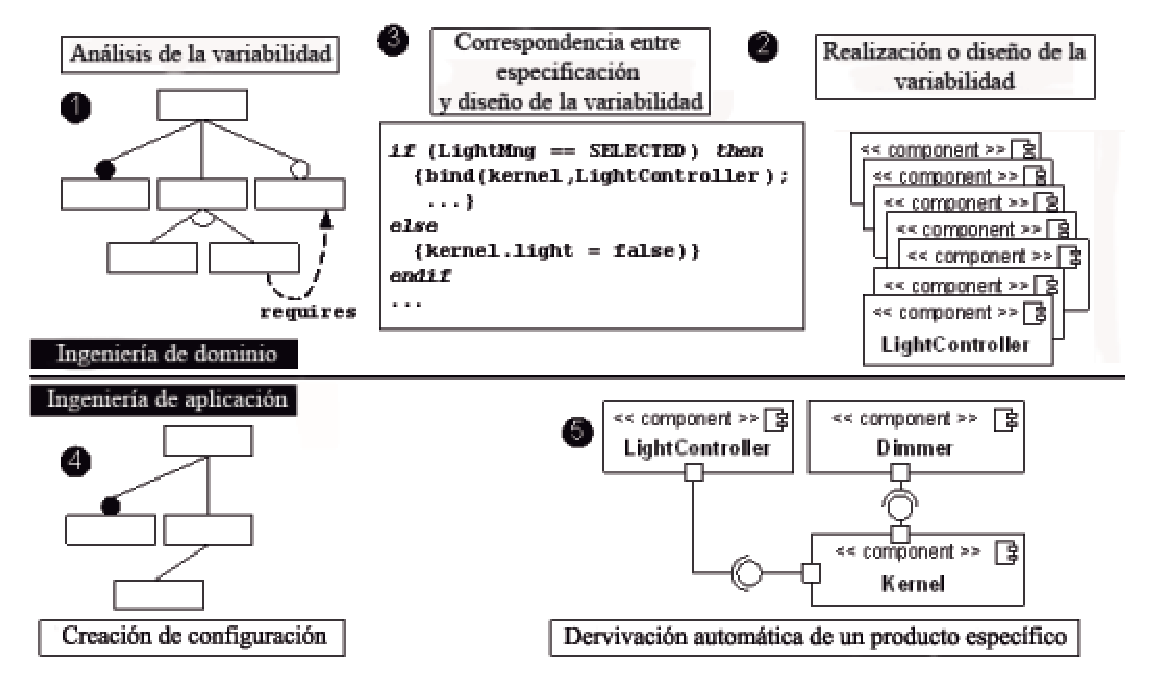
\includegraphics[width=.95\linewidth]{background/domainAplicationEngineering.eps} \\
  \caption{Proceso de desarrollo de una l�nea de productos software}
  \label{back:fig:domainAplicEng}
\end{figure}

En la fase de ingenier�a del dominio, el primer paso a realizar ser�a un an�lisis de qu� caracter�sticas de la familia de productos son variables y por qu� y c�mo son variables. Esta parte es la que se conoce como \emph{an�lisis o especificaci�n de la variabilidad} (Figura~\ref{back:fig:domainAplicEng}, punto 1). A continuaci�n, se ha de dise�ar una arquitectura o marco de trabajo para la familia de productos software que permita soportar dichas variaciones. Esta actividad se conoce como \emph{realizaci�n o dise�o de la variabilidad} (Figura~\ref{back:fig:domainAplicEng}, punto 2). El siguiente paso es establecer una serie de reglas que especifiquen como hay que instanciar la arquitectura previamente creada de acuerdo con las caracter�sticas seleccionadas por cada cliente. Esta fase es la que se conoce como \emph{correspondencia entre especificaci�n y dise�o de la variabilidad} (Figura~\ref{back:fig:domainAplicEng}, punto 3).

En la fase de ingenier�a de aplicaci�n, se crear�a una \emph{configuraci�n}, que no es m�s que una selecci�n de caracter�sticas que un usuario desea incluir en su producto (Figura~\ref{back:fig:domainAplicEng}, punto 4). En el caso ideal, usando esta configuraci�n, deber�amos poder ejecutar las reglas de correspondencia entre especificaci�n y dise�o de la variabilidad para que la arquitectura creada en la fase de ingenier�a del dominio se adaptase autom�ticamente generando un producto concreto espec�fico acorde a las necesidades concretas del usuario (Figura~\ref{back:fig:domainAplicEng}, punto 5). En caso no ideal, dichas reglas de correspondencia deber�n ejecutarse a mano, lo cual suele ser un proceso tedioso, largo, repetitivo y propenso a errores.

Este proyecto se centra en la primera etapa de este proceso de desarrollo, es decir en el an�lisis de la variabilidad de una familia de productos software mediante �rboles de caracter�sticas. La siguiente secci�n proporciona una breve pero completa descripci�n acerca del funcionamiento de los �rboles de caracter�sticas.


\section{�rboles de caracter�sticas}
\label{sec:back:fmodels}
%%==================================================================%%
%% Author : Tejedo Gonz�lez, Daniel                                 %%
%%          S�nchez Barreiro, Pablo                                 %%
%% Version: 1.0, 18/11/2012                                         %%                   
%% Version: 2.0, 05/02/2013                                         %%                   
%%                                                                  %%
%% Memoria del Proyecto Fin de Carrera                              %%
%% Antecedentes, �rboles de caracter�sticas                         %%
%%==================================================================%%

Como se ha comentado en la secci�n anterior, una de las tareas clave para el �xito de una l�nea de productos software consiste en analizar la variabilidad existente en la familia de productos software que dicha l�nea de productos software pretende cubrir. Aqu� es donde entran en juego los \emph{�rboles de caracter�sticas}~\cite{kang:1990, czarnecky:2005, danilo:2003}. Una \emph{caracter�stica} se define como ``\emph{un incremento en la funcionalidad del producto}'', o m�s formalmente, ``\emph{una caracter�stica es una propiedad de un sistema que es relevante a algunos \emph{stakeholders} y que es utilizada para capturar propiedades comunes o diferenciar entre sistemas de una misma familia}''~\cite{eisenecker:2000}. De este modo un producto queda representado por las caracter�sticas que posee.

Para poder capturar las divergencias y aspectos comunes entre los distintos productos de una misma familia, los �rboles de caracter�sticas organizan de forma jer�rquica el conjunto de caracter�sticas que posee una familia de productos. Cada caracter�stica se representa como un nodo en el �rbol de caracter�sticas. La ra�z de dicho �rbol es siempre el sistema o producto software cuya variabilidad estamos analizando. Cada caracter�stica se puede descomponer en varias subcaracter�sticas, siendo est�s �ltimas nodos \emph{hijos} de la primera caracter�stica, que actuar�a como \emph{padre}. Dependiendo de si dichas subcaracter�sticas son obligatorias, alternativas u opcionales, existen diversos tipos de relaciones padre-hijo. 

%%=========================================================================================%%
%% NOTA(Pablo): Para esta figura, hazte un modelo para la Smart Home sin habitaciones ni   %%
%%              plantas. Lo puedes encontrar en un art�culo que te mando luego             %% %%=========================================================================================%%
\begin{figure}[!tb]
    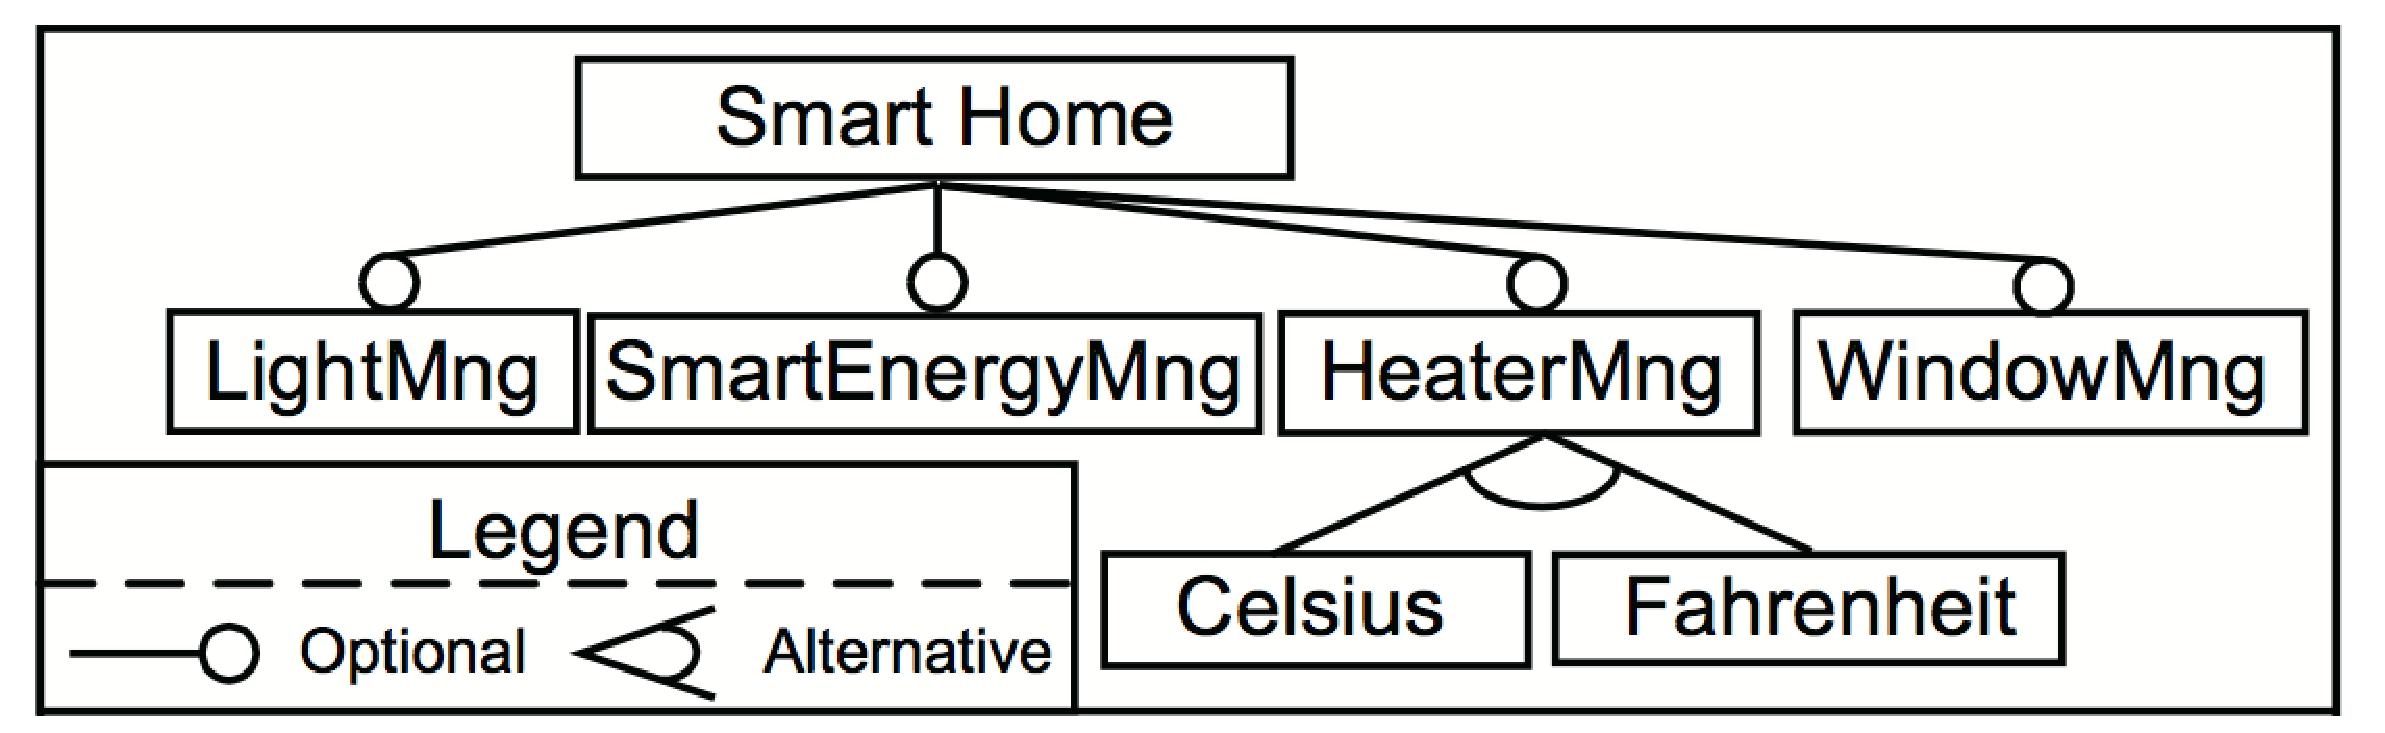
\includegraphics[scale=0.3]{background/simpleSmarthome.eps}
    \caption{�rbol de caracter�sticas simple para nuestro caso de estudio}
    \label{fig:smartHomeFMsimple}
\end{figure}

La Figura~\ref{fig:smartHomeFMsimple} muestra como ejemplo un �rbol de caracter�sticas que especifica la variabilidad inherente a nuestro caso de estudio, sin considerar que las plantas y habitaciones puedan configurarse de manera individual. El �rbol representa un hogar inteligente definido por las siguientes caracter�sticas: controlador de luz, controlador de temperatura, controlador de ventanas y controlador de la energ�a. Tal como se puede ver en la leyenda de la figura, todas estas caracter�sticas son opcionales, es decir, podemos decidir si queremos que est�n o no presentes en el hogar inteligente que generemos. Adem�s, para la caracter�stica ''controlador de temperatura" se ha de especificar una de las dos opciones alternativas que se plantean: grados celsius o grados fahrenheit.

El modo de representaci�n de los �rboles de caracter�sticas permite especificar cierto tipo de restricciones que pueden resultar necesarias para representar con exactitud el comportamiento del producto que queramos construir. En el caso de la Figura~\ref{fig:smartHomeFMsimple} se puede observar que mediante las relaciones ya se est� modelando la restricci�n que especifica que el controlador de temperatura ha de ser necesariamente de uno de los tipos que se indican en el modelo. Otros tipos de relaciones que pueden incluirse sirven para especificar otras restricciones, por ejemplo la obligatoriedad de seleccionar una caracter�stica o un grupo de ellas.

Sin embargo, si quisi�ramos incluir algunas restricciones m�s complejas, la representaci�n gr�fica de los �rboles de caracter�sticas se queda corta. Por ejemplo, en la Figura~\ref{fig:smartHomeFMsimple} podr�amos querer especificar la restricci�n de que si nuestro hogar inteligente tiene un controlador de energ�a, ha de tener tambi�n un controlador de calefacci�n en grados celsius. Es imposible modelar esta restricci�n con las herramientas de las que los �rboles de caracter�sticas disponen. Es por ese motivo que debe permitirse la posibilidad de especificar restricciones externas al �rbol mediante alg�n tipo de lenguaje textual o gr�fico.

%%=========================================================================================%%
%% NOTA(Pablo): Explicar el modelo creado, indicando las cosas que son variables, las que  %%
%%              son alternativas, etc.                                                     %%
%%              Explicar el problema de las restricciones externas                         %%
%%=========================================================================================%%

\begin{figure}[!tb]
    \centerline{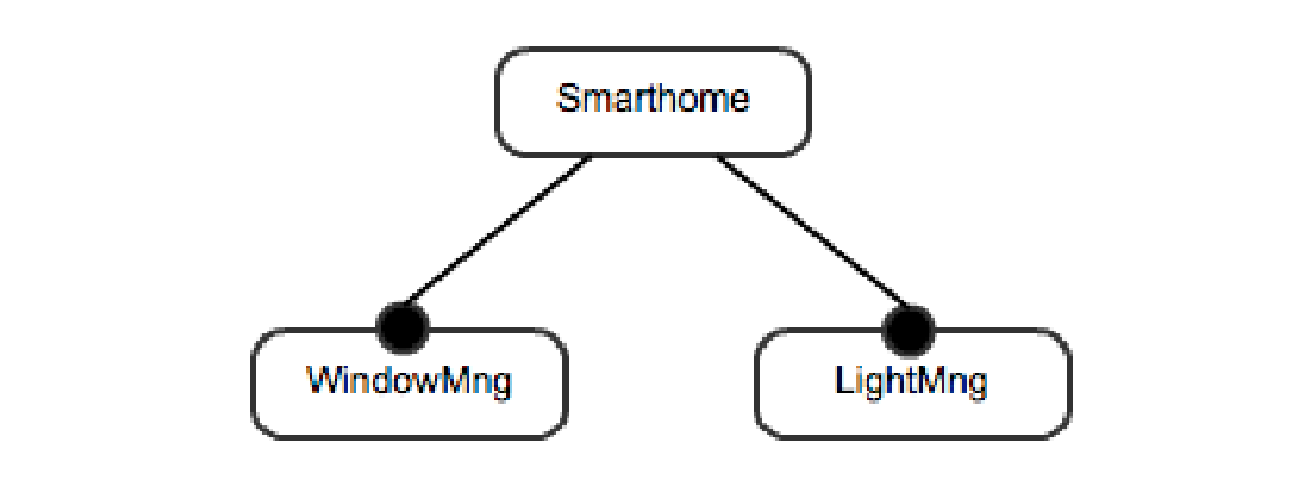
\includegraphics[scale=0.3]{background/simpleSmarthomeConf.eps}}
    \caption{Configuraci�n para la versi�n sencilla del caso de estudio}
    \label{fig:smartHomeConfSimple}
\end{figure}

Una vez creado un �rbol de caracter�sticas para una l�nea de productos software, podemos indicar las caracter�sticas que podemos incluir en un producto software concreto mediante la creaci�n de configuraciones. Una \emph{configuraci�n} no es m�s que una selecci�n v�lida de caracter�sticas. La Figura~\ref{fig:smartHomeConfSimple} muestra en un ejemplo de configuraci�n para el modelo de la Figura~\ref{fig:smartHomeFMsimple} donde se indica que el producto que deseamos construir debe incluir �nica y obligatoriamente un dispositivo de control de luz y un dispositivo de control de ventanas. Obviamente, dicho modelo debe satisfacer las restricciones externas declaradas. 

Los �rboles de caracter�sticas como los anteriormente expuestos no permiten modelar que pueda existir un n�mero variable de ciertas caracter�sticas, como, en nuestro caso, de plantas y habitaciones, y que, adem�s, cada instancia particular de una caracter�sticas pueda  configurarse de forma distinta. Por ejemplo, podr�amos decidir que el sal�n de la casa tenga control inteligente de temperatura, mientras que la cocina, que est� sometida a mayores variaciones de temperatura, no contenga dicha caracter�sticas. Para solventar esta carencia, se introdujeron en los �rboles de caracter�sticas el concepto de caracter�stica clonable. 

\begin{figure}[!tb]
    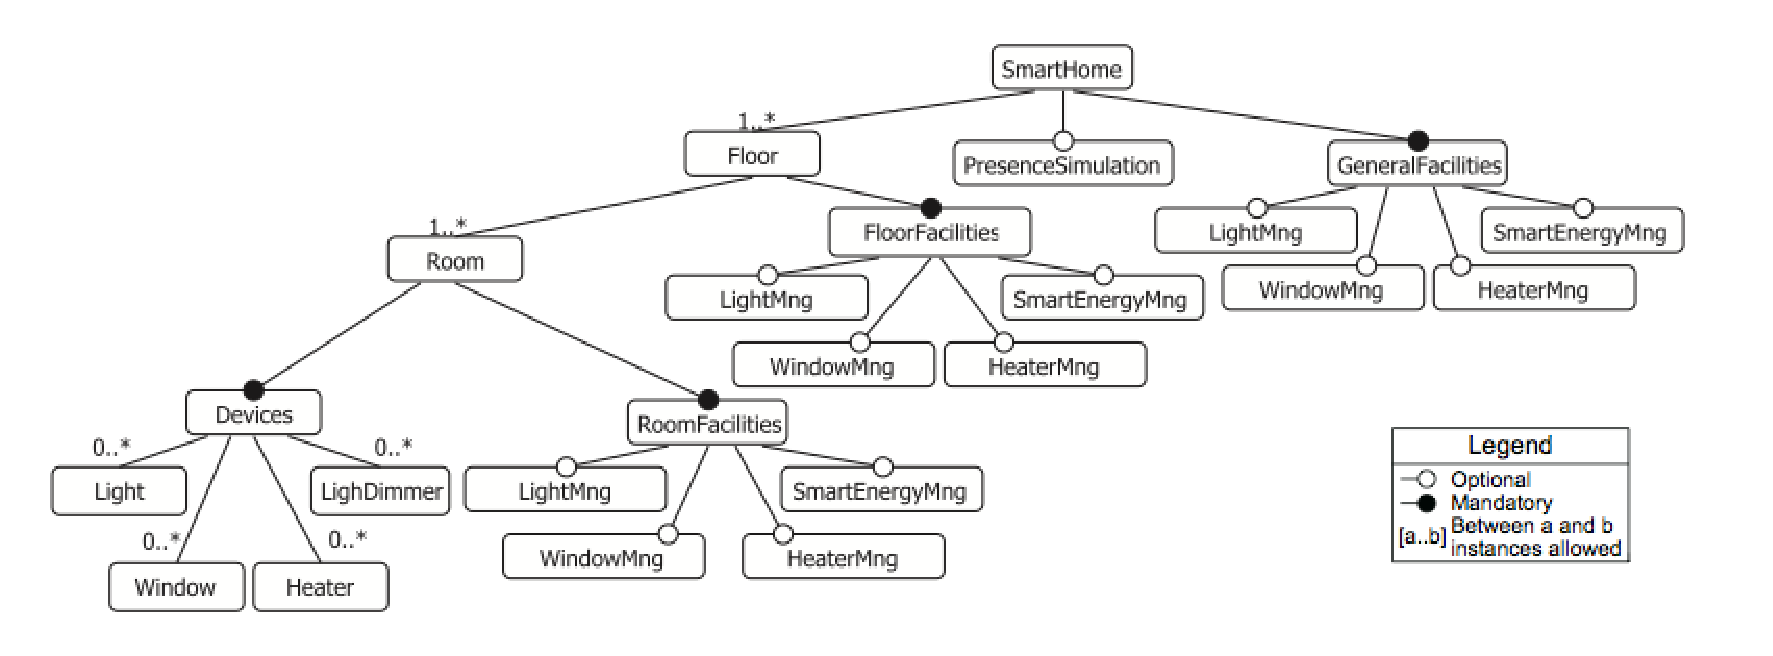
\includegraphics[scale=0.4]{background/featuremodel.eps}
    \caption{�rbol de caracter�sticas completo para nuestro caso de estudio}
    \label{fig:smarHomeFeatureModel}
\end{figure}

La Figura~\ref{fig:smarHomeFeatureModel} muestra el �rbol de caracter�sticas para nuestro caso de estudio incluyendo \emph{caracter�sticas clonables}. Las caracter�sticas \emph{Floor} (Piso) y \emph{Room} (Habitaci�n) son clonables porque pueden aparecer m�s de una vez en las configuraciones creadas. La cardinalidad de ambas caracter�sticas es 1..*, lo que significa que pueden ser seleccionadas de una a infinitas veces. As� mismo, cualquier caracter�stica que sea hija de ellas directa o indirectamente es considerada inmediatamente como caracter�stica. Este es el caso, por ejemplo, de \emph{Devices} y de sus caracter�sticas hijas (\emph{Heater}, \emph{Window}, etc.), que son consideradas clonables tanto por su cardinalidad como por ser hijas de una caracter�stica clonable. 

La repetici�n de las caracter�sticas correspondientes a los diversos controladores (es decir, \emph{WindowMng}, \emph{HeaterMng}, etc.) se debe a que gracias a las caracter�sticas clonables ahora podemos diferenciar los controladores seg�n su colocaci�n y alcance. Es decir, el controlador de temperatura hijo de \emph{RoomFacilities} afectar� s�lo a la habitaci�n a la que pertenezca, el hijo de \emph{FloorFacilities} afectar� al piso al que pertenezca, y el hijo de \emph{GeneralFacilities} afectar� a todo el hogar creado. 
%%=========================================================================================%%
%% NOTA(Pablo): A�adir la figura, si no te entrase bien a lo ancho, mira como meterla 
%%              apaisada en Latex.
%%=========================================================================================%%

A la hora de crear configuraciones para este nuevo �rbol hay que tener en cuenta que podemos seleccionar en m�s de una ocasi�n ciertas caracter�sticas, por lo que necesitamos valernos de alg�n mecanismo que nos permita diferenciarlas entre ellas. El modo de lograrlo es poniendo un nombre a las diferentes selecciones o clones que hagamos de una misma caracter�stica. 

La Figura~\ref{fig:smarthomeCompleteConf} muestra un ejemplo de configuraci�n para el �rbol de caracter�sticas con caracter�sticas clonables de la Figura~\ref{fig:smarHomeFeatureModel}. En ella se puede apreciar que se diferencia entre las diferentes selecciones de la caracter�stica \emph{Floor} poni�ndoles un nombre, en este caso \emph{Ground} (Planta Baja) y \emph{First} (Primer Piso). Del mismo modo con las habitaciones \emph{Kitchen} (Cocina) y \emph{Living} (Sal�n), pertenecientes a la planta baja, y \emph{Bed} (Dormitorio), perteneciente al primer piso. Observando el �rbol de la figura es sencillo comprender qu� elementos y/o controladores tiene instalados cada estancia. Por ejemplo, la cocina est� dotada de dos luces, un regulador de luz, una ventana, un controlador de luz y un controlador de ventanas.

%%=========================================================================================%%
%% NOTA(Pablo): Explicar como se configuran las caracter�sticas clonables usando un 
%%              ejemplo
%%=========================================================================================%%

Como en el caso anterior, las diversas configuraciones no s�lo han de cumplir las restricciones impuestas por el propio �rbol de caracter�sticas, sino tambi�n las restricciones externas. Pero debido a la presencia de caracter�sticas clonables ahora existe un abanico mucho mayor de restricciones posibles que definir. Del mismo modo que antes se pod�an definir diversas restricciones l�gicas ($a implies b$), la presencia de caracter�sticas clonables hace que tambi�n sean necesarias las restricciones num�ricas ($a >= b$), lo que tambi�n a�ade la dificultad de diferenciar qu� caracter�sticas pueden realizar operaciones l�gicas y cuales no. 

Tambi�n es necesaria una operaci�n de contexto que permita aplicar estas restricciones s�lamente a sub�rboles de la configuraci�n. Esto es imprescindible para definir una restricci�n que, por ejemplo, valide que si una habitaci�n tiene un controlador de ventanas, forzosamente ha de tener instalada al menos una ventana. Sin la operaci�n de contexto ser�a imposible saber a qu� caracter�stica \emph{WindowMng} en concreto est� haciendo referencia la restricci�n definida.

El objetivo de este proyecto es implementar un lenguaje textual que haga posible la definici�n de restricciones externas para �rboles de caracter�sticas con caracter�sticas clonables con todas las peculiaridades definidas anteriormente, as� como una herramienta que permita validar si las configuraciones creadas satisfacen o no esas restricciones. 
%%=========================================================================================%%
%% NOTA(Pablo): Explicar el problema de las restricciones cuando incluyen caracter�sticas
%%              clonables y decir que implementar un lenguaje para resolver ese problema 
%%              es el objetivo de este proyecto
%%=========================================================================================%%

%%=========================================================================================%%
%% NOTA(Pablo): Esto no se entiende de forma clara, por lo que se suprime                                         %%
%%=========================================================================================%%
%%
%% Por otro lado, un modelo de caracter�sticas debe poder representar la cardinalidad de 
%% las caracter�sticas, por motivos tanto de comprensi�n (es mucho mejor contar con un 
%% �rbol de 8 nodos que con uno de 100, teniendo ambos un significado equivalente), como 
%% de funcionalidad, ya que permite expresar ciertas restricciones que de no contar con 
%% la cardinalidad no podr�an expresarse.
%% 
%% Adem�s se podr�n disponer de restricciones de usuario m�s complejas, que son las que
%% se han implementado en el editor de especificaci�n y validaci�n de restricciones 
%% desarrollado en este proyecto.
%%
%%=========================================================================================%%

%%=========================================================================================%%
%% NOTA(Pablo): Esto queda obsoleto en el nuevo esquema, por lo cual se suprime            %%
%%=========================================================================================%%
%%
%% La figura \ref{fig7} muestra un ejemplo de modelo de caracter�sticas. En este caso se 
%% trata de un modelo de una casa inteligente o SmartHome, a trav�s del cual, 
%% seleccionando ciertas caracter�sticas u otras podremos construir qu� tipo de casa 
%% queremos. Cada una de las m�ltiples casas diferentes que podamos construir es lo que 
%% se denonima una especializaci�n o configuraci�n de nuestro modelo de caracter�sticas.
%% 
%%  El proceso de crear una configuraci�n a partir de un modelo de caracter�sticas se 
%% conoce como proceso de configuraci�n o proceso de especializaci�n. Consiste en 
%% transformar un modelo de caracter�sticas de tal forma que el modelo resultante sea un
%%  subconjunto de las posibles configuraciones denotadas por el primer modelo. La figura 
%% \ref{fig8} muestra una posible configuraci�n para el modelo de caracter�sticas de la figura %% \ref{fig7}.
%%
%% La relaci�n entre un diagrama de caracter�sticas y una configuraci�n es an�loga a la
%% existenteentre una clase y una de sus instancias en programaci�n orientada a objetos.
%%
%%=========================================================================================%%

\begin{figure}[!tb]
    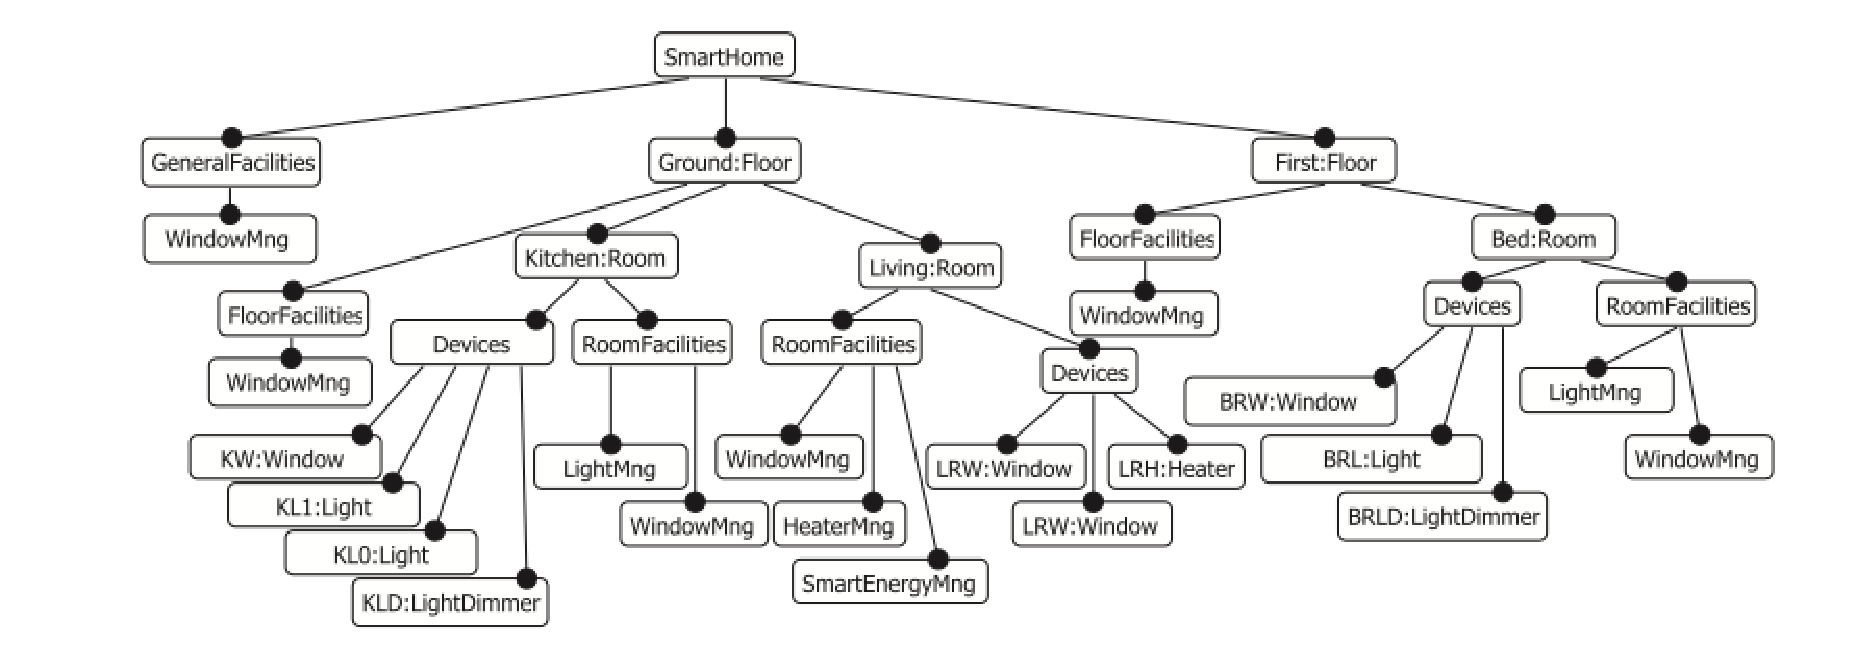
\includegraphics[scale=0.4]{background/configuration.eps}
    \caption{Posible modelo de configuraci�n de una casa inteligente concreta}
    \label{fig:smarthomeCompleteConf}
\end{figure}

\begin{figure}[!tb]
    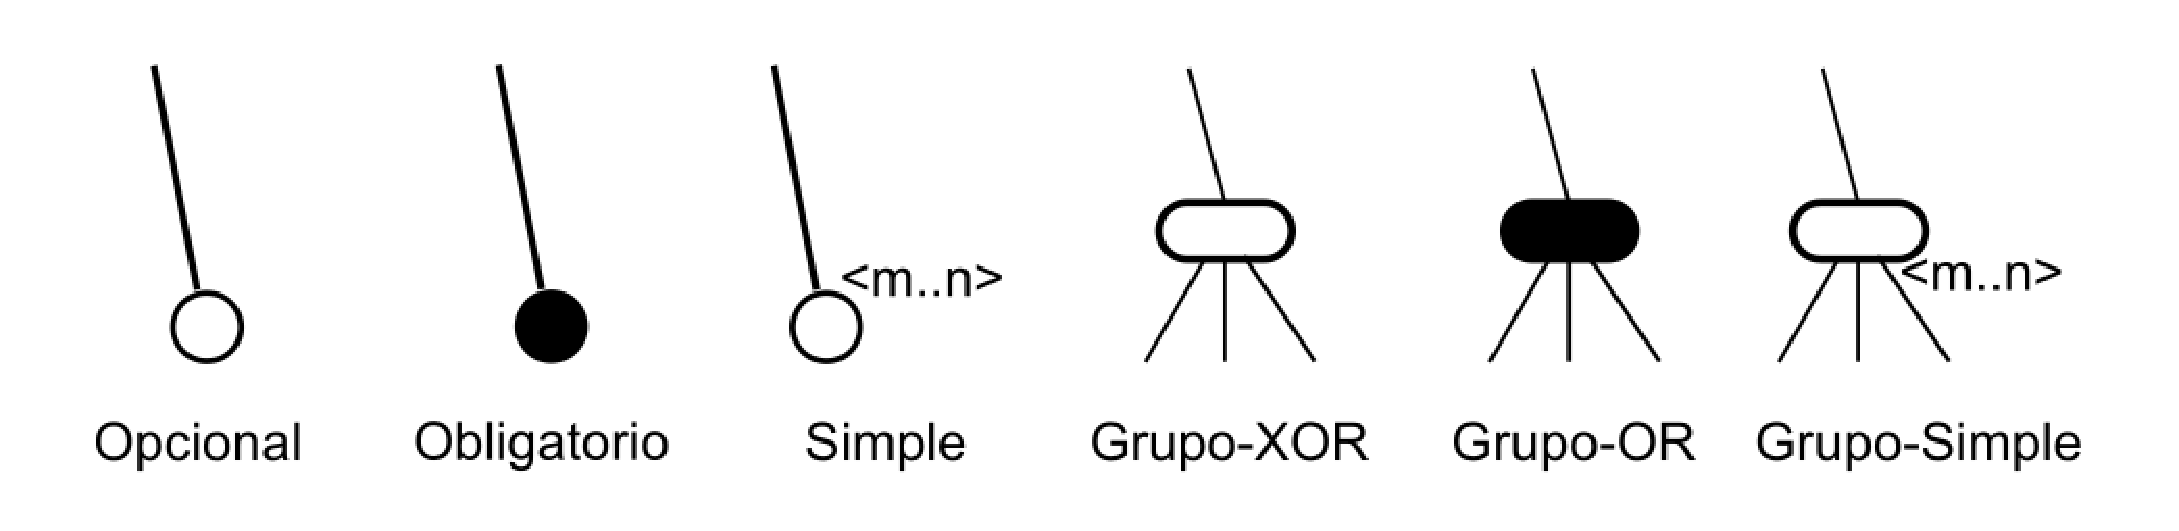
\includegraphics[scale=0.35]{background/relations.eps}
    \caption{Tipos de relaciones entre caracter�sticas }
    \label{fig:relacionesFeatures}
\end{figure}

A modo de resumen, la Figura~\ref{fig:relacionesFeatures} muestra las posibles relaciones que pueden entre caracter�sticas, as� como su representaci�n gr�fica. Dichas relaciones se describen a continuaci�n:

\begin{description}
    \item[Opcional] La caracter�stica hija puede estar o no estar seleccionada
    \item[Obligatoria] La caracter�stica siempre debe estar seleccionada.
    \item[Clonable] La caracter�stica tendr� una cardinalidad $<m,n>$, siendo m y n n�meros enteros que denotan el m�nimo y el m�ximo respectivamente de caracter�sticas que podemos seleccionar.
    \item[Grupo-xor] S�lo una de las caracter�sticas pertenecientes al grupo puede ser seleccionada.
    \item[Grupo-or] Debemos seleccionar como m�nimo una de las subcaracter�sticas, pudiendo seleccionar m�s si lo deseamos.
    \item[Grupo con cardinalidad] El n�mero m�nimo y m�ximo de caracter�sticas a seleccionar dentro del grupo vendr� determinado por su cardinalidad $<m,n>$.
\end{description}

Tras esta secci�n se han proporcionado al lector lo necesario para comprender el contexto del problema que este Proyecto Fin de Carrera pretende resolver. Las siguientes secciones est�n destinadas a explicar las tecnolog�as concretas que se han utilizado para implementar el lenguaje que da soluci�n a los problemas planteados. 


\section{\emph{Eclipse Modelling Framework}}
\label{sec:back:ecore}
%%==================================================================%%
%% Author : Tejedo Gonz�lez, Daniel                                 %%
%%          S�nchez Barreiro, Pablo                                 %%
%% Version: 1.0, 18/11/2012                                         %%                  
%%                                                                  %%
%% Memoria del Proyecto Fin de Carrera                              %%
%% Antecedentes, ecore                                              %%
%%==================================================================%%

EMF \emph{Eclipse Modeling Framework}~\cite{} es un \emph{plug-in} para Eclipse~\cite{} que permite elaborar metamodelos. Pera ello proporciona un lenguaje de metamodelo denominado Ecore, el cual se ha convertido en el est�ndar de factor para la realizaci�n de metamodelos. Utilizando Ecore se pueden crear metamodelos de forma gr�fica usando una notaci�n muy similar a la los diagramas de clases de UML. La Figura~\ref{fig:sle:metamodeloGrafo} muestra un sencillo ejemplo de metamodelo en Ecore (ver Secci�n~\ref{sec:intr:sle} para m�s detalles). EMF tambi�n incorpora una herramienta para la validaci�n reglas adicionales que no puedan ser especificadas a nivel de del metamodelo. 
 
EMF permite que, a partir de un metamodelo especificado en Ecore, podamos, utilizando diversos generadores de c�digo, crear autom�ticamente un conjunto de clases que nos permiten manipular dichos modelos a nivel de c�digo. Dichas clases se pueden adem�s distribuir como \emph{plug-in} para el entorno Eclipse.

Adem�s, al haberse convertido en est�ndar \emph{de facto} para el desarrollo de metamodelos, Ecore es compatible con multitud de herramientas para Ingenier�a de Lenguajes Dirigida por Modelos, como EMFText, la cual se describe en la siguiente secci�n, o diversos generadores de c�digo o herramientas de transformaci�n de modelos. 



\section{EMFText}
\label{sec:back:emftext}
%%==================================================================%%
%% Author : Tejedo Gonz�lez, Daniel                                 %%
%%          S�nchez Barreiro, Pablo                                 %%
%% Version: 1.0, 18/11/2012                                         %%                   %%                                                                  %%
%% Memoria del Proyecto Fin de Carrera                              %%
%% Antecedentes, emftext                                      %%
%%==================================================================%%


EMFText es una herramienta espec�ficamente dise�ada para dise�ar las gram�ticas de los lenguajes que hayan sido dise�ados previamente con un metamodelo de Ecore. Est� especializado para la creaci�n de Lenguajes Espec�ficos de Dominio, aunque tambi�n se pueden crear lenguajes de prop�sito general. 

Pero, como en casi todos los casos de este tipo de herramientas, su mayor virtud es la enorme cantidad de c�digo autogenerado que produce, y que elimina al programador de tareas tediosas que adem�s en muchos casos podr�an resultar complicadas. Todo el c�digo generado es completamente independiente de EMFText, es decir, podr� ser ejecutado en plataformas que no tengan la herramienta instalada. 

Todo el c�digo generado por EMFText est� dise�ado de tal modo que sea f�cil de modificar en caso de que queramos poner en pr�ctica algunas funcionalidades poco habituales. Se facilita mucho la labor a la hora de modificar estructuras como el postprocesador de nuestra gram�tica. Todas las gram�ticas construidas tendr�n que ser LL por defecto, a no ser que queramos modificar los parsers generados, posibilidad tambi�n disponible. 

Otro tipo de funcionalidades implementadas, quiz�s no tan importantes pero tambi�n de gran utilidad, son el coloreado de c�digo (por defecto o personalizable), funci�n de completar c�digo, generaci�n del �rbol parseado en el la vista de eclipse Outline o generaci�n de c�digo para crear un depurador para nuestro lenguaje.

\begin{figure}[t]
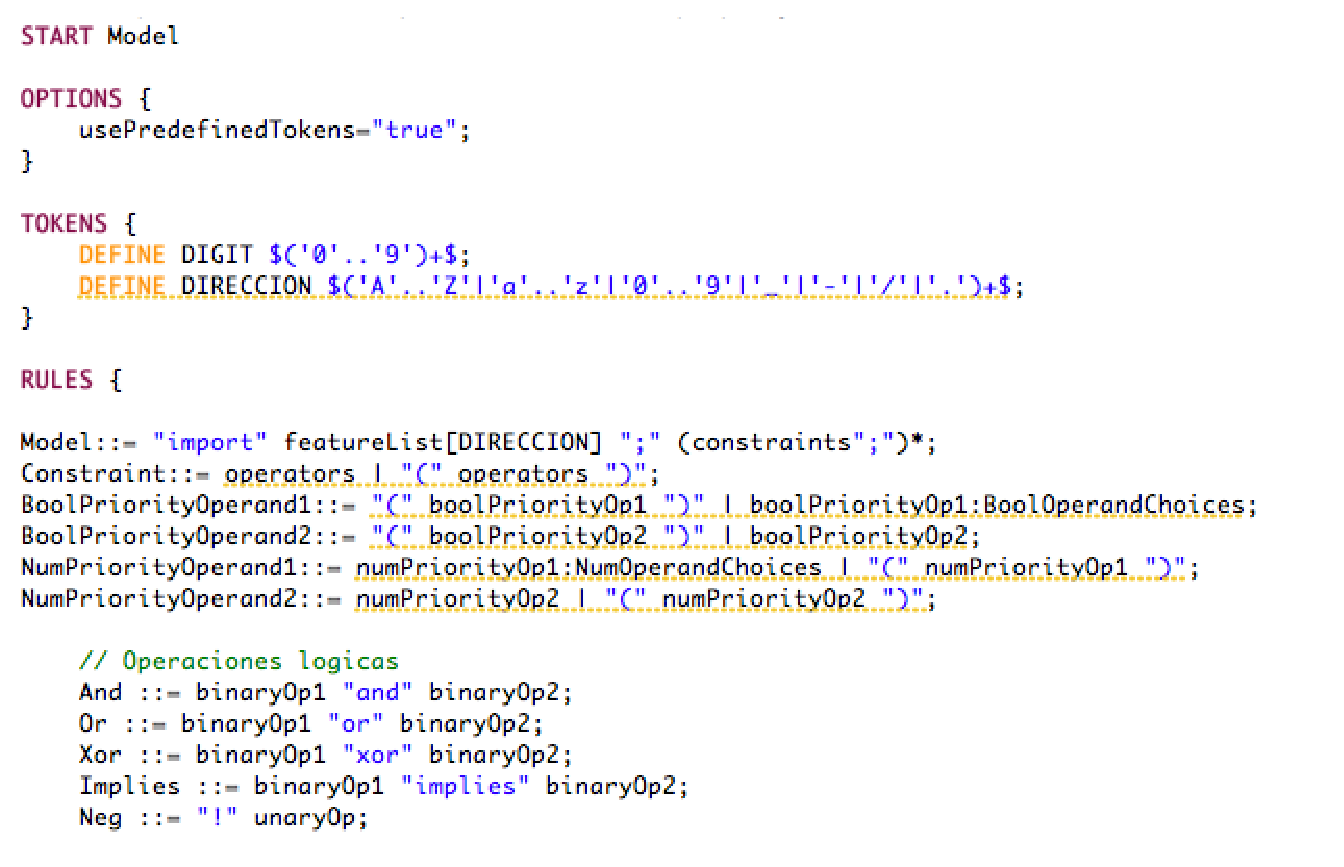
\includegraphics[scale=0.5]{background/gramatica.eps}
\caption{Trozo de la gram�tica de nuestro editor de especificaci�n y validaci�n de restricciones}
\label{fig5}
\end{figure}


EMFText permite la definici�n de gram�ticas utilizando un lenguaje est�ndar para la definici�n de expresiones regulares, adem�s de incorporar algunas particularidades propias que facilitan ciertas tareas. En la figura \ref{fig5} se muestra una peque�a captura que contiene una porci�n de la gram�tica construida para nuestro editor de especificaci�n y validaci�n de restricciones. 

\section{Arquitectura de plugins de Eclipse}
\label{sec:back:eplugins}
%%==================================================================%%
%% Author : Tejedo Gonz�lez, Daniel                                 %%
%%          S�nchez Barreiro, Pablo                                 %%
%% Version: 1.0, 18/11/2012                                         %%                   
%% Version: 1.0, 06/02/2013                                         %%                   
%%                                                                  %%
%% Memoria del Proyecto Fin de Carrera                              %%
%% Antecedentes, arquitectura de plugins de eclipse                 %%
%%==================================================================%%

El entorno de desarrollo Eclipse es un ejemplo de arquitectura modular f�cilmente extensible mediante una compleja, pero sencilla para el programador, arquitectura de \emph{plug-ins}. Un \emph{plug-in} en Eclipse es un componente que provee un cierto tipo de servicio dentro del contexto del espacio de trabajo de Eclipse. Es decir, una herramienta que se puede integrar en el entorno Eclipse junto con sus otras funcionalidades. Dado que la herramienta \emph{Hydra} fue dise�ada como un \emph{plug-in} para Eclipse, y nuestro editor pretende integrarse tanto en \emph{Hydra} como en \emph{Eclipse}, es necesario conocer y manejar el funcionamiento de la arquitectura de plug-ins de Eclipse.

Aunque la arquitectura de plug-ins de Eclipse tiene mucha profundidad y ofrece muchas posibilidades, es imprescindible el dominio de dos de sus conceptos clave para poder trabajar con ella: las dependencias y los puntos de extensi�n. Mediante las dependencias podemos indicar que el plug-in a desarrollar tiene que incorporar toda la funcionalidad y estructura de otro plug-in (en este caso nuestro editor tiene, entre otras, una dependencia con el plug-in de la herramienta Hydra original). Un punto de extensi�n permite a�adir cierta funcionalidad al plug-in desarrollado mediante la inclusi�n autom�tica de ciertos segmentos de c�digo. Un ejemplo cl�sico de punto de extensi�n, y que adem�s ha sido utilizado en el transcurso de este proyecto, es el que permite a�adir un bot�n a la barra de tareas de Eclipse de manera autom�tica, teniendo que implementar �nicamente el c�digo del manejador de ese bot�n.

 \begin{figure}[!tb]
    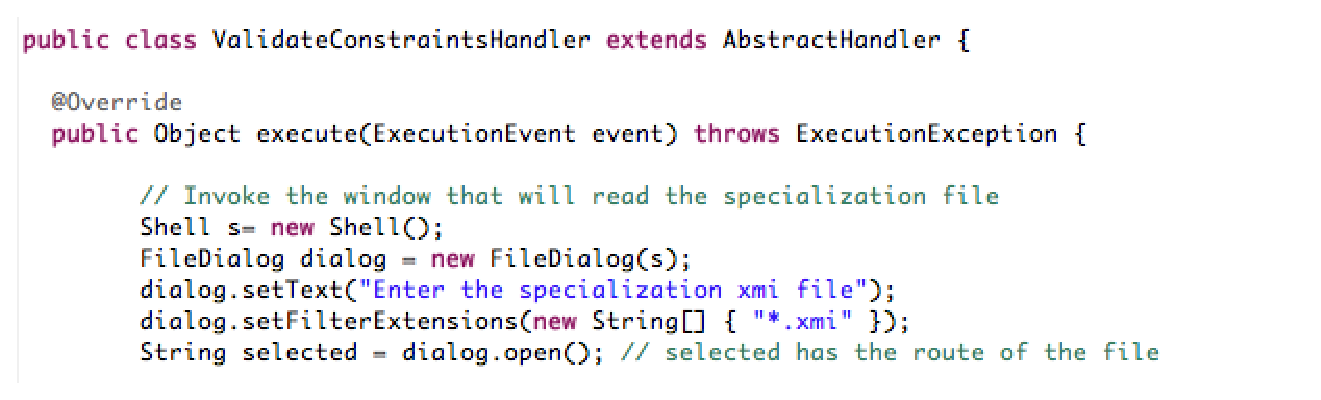
\includegraphics[scale=0.4]{background/codigoManejador.eps}
    \caption{Trozo de c�digo del manejador de un bot�n introducido mediante un punto de extensi�n}
    \label{fig:codigoManejador}
\end{figure}

%%==============================================================================================%%
%% NOTA(Pablo): Esto no se entiende nada
%%==============================================================================================%%
%%
%% En particular, se han utilizado mucho los puntos de extensi�n. Un punto de extensi�n en un
%% plug-in indica la posibilidad de que ese plug-in sea a su vez parte de otro, o que haya 
%% otros plug-ins que sean parte de �l. Esta particularidad permite no s�lo la integraci�n de 
%% nuestro editor con Hydra, sino tambi�n la personalizaci�n de men�s y botones para �l 
%% gracias a la creaci�n de puntos de extensi�n con plug-ins de creaci�n de men�s y barras de
%% herramientas.
%%
%%==============================================================================================%%

%%==============================================================================================%%
%% NOTA(Pablo): Para solucionar
%% - Describir en uno o dos p�rrafos c�mo funciona la arquietctura de plug-ins para Eclipse
%% - Poner un ejemplo de punto de extensi�n, sencillo y concreto, y explicar como funciona 
%%   el punto de extensi�n utilizando algo de c�digo.
%% Si no sabes como escribir esta secci�n, la eliminas directamente, y actualizas la intro 
%% al Cap�tulo de forma conveniente.
%%==============================================================================================%%


\section{Sumario}
\label{sec:back:sumario}
%%==================================================================%%
%% Author : Tejedo Gonz�lez, Daniel                                 %%
%%          S�nchez Barreiro, Pablo                                 %%
%% Version: 1.0, 25/11/2012                                         %%                   
%%                                                                  %%
%% Memoria del Proyecto Fin de Carrera                              %%
%% Sintaxis abstracta, sumario                          %%
%%==================================================================%%

Durante el presente cap�tulo se ha descrito el proceso de definici�n de la sintaxis abstracta de nuestro lenguaje. Este proceso abarca subtareas como la captura de requisitos del lenguaje, la creaci�n de un metamodelo que permita la creaci�n de sintaxis concretas apropiadas, la validaci�n de restricciones externas a ese metamodelo, y las pruebas que corroboren que todos los elementos creados funcionan correctamente. En el siguiente cap�tulo profundizaremos acerca del dise�o de la gram�tica para nuestro lenguaje, as� como de las herramientas utilizadas para implementar esa gram�tica.


% Cap�tulo 3: Creaci�n de la sintaxis abstracta
%%==================================================================%%
%% Author : Tejedo Gonz�lez, Daniel                                 %%
%%          S�nchez Barreiro, Pablo                                 %%
%% Version: 1.0, 25/11/2012                                         %%                   %%                                                                  %%
%% Memoria del Proyecto Fin de Carrera                              %%
%% Sintaxis abstracta, archivo ra�z                                       %%
%%==================================================================%%

\chapterheader{Creaci�n de la sintaxis abstracta}{Creaci�n de la sintaxis abstracta}
\label{chap:metamodelo}

A partir de aqu�, los siguientes cap�tulos tratan de describir en detalle cada una de las tareas expuestas en la planificaci�n del proyecto. Evidentemente, se ha obviado la tarea de documentaci�n, pues no requiere explicaci�n alguna. Este cap�tulo en concreto versa sobre la creaci�n de la sintaxis abstracta del lenguaje, as� como cada una de las subtareas subyacentes.

\chaptertoc

\section{Captura de requisitos}
\label{sec:meta:requisitos}
%%==================================================================%%
%% Author : Tejedo Gonz�lez, Daniel                                 %%
%%          S�nchez Barreiro, Pablo                                 %%
%% Version: 1.0, 25/11/2012                                         %%
%% Version: 2.0, 06/02/2013                                         %%
%%                                                                  %%
%% Memoria del Proyecto Fin de Carrera                              %%
%% Sintaxis abstracta, requisitos                                   %%
%%==================================================================%%

El primer paso para desarrollar nuestro lenguaje era conocer qu� aspecto deb�a tener nuestro lenguaje y qu� restricciones deb�a satisfacer. Es decir, en primer lugar debemos realizar un proceso que podemos denominar de captura de requisitos para poder comprender qu� es lo que tiene que hacer exactamente el lenguaje que se pretende crear.

Concretamente nuestro lenguaje hab�a sido pr�cticamente definido por el profesor Pablo S�nchez, del Departamento de Matem�ticas, Estad�stica y Computaci�n de la Universidad de Cantabria, mediante notaci�n BNF. Las ideas subyacentes a dicho lenguaje son las que se describen a continuaci�n.

%%==================================================================%%
%% NOTA(Pablo): Aqu� traduce la secci�n III del art�culo que te
%%              env�o adjunto. Si te hacen falta las fuentes del
%%              art�culo, me las pides.
%%
%%              Traduce primero del ingl�s y luego lo repasas y lo
%%              reescribes para que suene a castellano
%% 
%%              Si en la secci�n III no aparecen las razones por 
%%              las cuales una caracter�stica es clonable, buscar 
%%              en qu� parte del art�culo aparecen y explicarlo

%%==================================================================%%

Adem�s nuestro lenguaje deb�a permitir vincular un un modelo de caracter�sticas sobre el cual se definir�n un conjunto de restricciones externas. Este modelo se utilizar�, por ejemplo, para comprobar que los s�mbolos que aparecen como nombres de caracter�sticas en las restricciones se refieren a caracter�sticas que realmente existen en el �rbol de caracter�sticas. Por ejemplo, una restricci�n del tipo $AdvancedHeating => Heating$ carecer�a de sentido si algunas de las caracter�sticas $AdvancedHeating$ o $Heating$ no apareciesen en el �rbol de caracter�sticas sobre el cual estamos definiendo restricciones.

%%======================================================================================%%
%% NOTA(Pablo): Esto posiblemente sobre al introducir la traducci�n de la Secci�n III.
%%              Si es as�, eliminarla.
%%              Si los conceptos de restricci�n con contexto y operaci�n cuantificada
%%              no apareciesen, meter esta clasificaci�n pero resumida
%%======================================================================================%%
%%
%% De entre todos esos requisitos b�sicos, es necesario entrar en detalle en el n�mero 3
%% y enumerar la lista de operaciones que pueden ser definidas por nuestro lenguaje. Se
%% pueden clasificar en los siguientes tipos: \\
%%
%% - L�gicas: Son operaciones cuyos operandos han de ser caracter�sticas sin
%%   cardinalidad (tambi�n llamadas caracter�sticas simples), y que se evaluan a
%%   verdadero o falso. Entre las operaciones l�gicas encontramos las cl�sicas not,
%%   and, or, xor e implica.
%%
%% - Num�ricas: Sus operandos han de ser caracter�sticas con cardinalidad (tambi�n
%%   llamadas caracter�sticas m�ltiples) o simplemente n�meros. Su resultado se evalua
%%   con un valor num�rico. Las operaciones num�ricas a implementar son la suma, resta,
%%   multiplicaci�n y divisi�n.
%%
%% - Comparativas: Sus operandos han de ser caracter�sticas m�ltiples o simplemente n�meros,
%%   pero su resultado se evalua con un valor booleano. Las operaciones de comparaci�n a
%%   implementar son igual que, mayor que, menor que, distinto que, mayor o igual que y menor
%%   o igual que.
%%
%% - Operaci�n de contexto: Operaci�n que permite hacer referencia a una caracter�stica
%%   hija de otra caracter�stica. Esta operaci�n tiene sentido para seleccionar
%%   caracter�sticas cuyo nombre pueda estar repetido pero que tengan contextos diferentes.
%%   Por ejemplo, en el modelo de caracter�sticas SmartHome de la figura \ref{figsmarthome}
%%   podemos observar que la caracter�stica HeaterMng est� presente en muchos contextos
%%   diferentes. Esta operaci�n es necesaria para poder saber con seguridad a cual de esos
%%   contextos estamos aplicando la restricci�n.
%%
%% - Operaci�n de selecci�n: Operaci�n que corresponde a los operadores l�gicos cl�sicos
%%   "para todo" o "existe", y que tiene la misma funcionalidad. Evalua si una restricci�n
%%   se cumple para todos los casos en que puede existir  o si se cumple en alguno de los
%%   casos. Por ejemplo, en el modelo de la figura \ref{figsmarthome} se podr�a evaluar una
%%   restricci�n para cada una de las habitaciones que hayan sido definidas, y saber si se
%%  cumple en todas, en alguna o en ninguna.
%%
%%======================================================================================%%

Utilizando esta informaci�n como base, procedimos a crear el correspondiente metamodelo en Ecore para nuestro lenguaje.




\section{Creaci�n del metamodelo}
\label{sec:meta:creacion}
%%==================================================================%%
%% Author : Tejedo Gonz�lez, Daniel                                 %%
%%          S�nchez Barreiro, Pablo                                 %%
%% Version: 1.0, 25/11/2012                                         %%                   %%                                                                  %%
%% Memoria del Proyecto Fin de Carrera                              %%
%% Sintaxis abstracta, creacion metamodelo                                      %%
%%==================================================================%%

Una vez hemos definido cuales son los requisitos del lenguaje, tenemos que construir nuestro metamodelo de tal modo que se ajuste a ellos y sea capaz de cumplirlos. El requisito m�s complejo y que requerir� m�s desaf�os de dise�o es, evidentemente, el de implementar todas las operaciones. As� que empezaremos primero por las partes m�s f�ciles.

Todas las restricciones que sean definidas en cada sintaxis concreta han de ser aplicadas al mismo modelo de caracter�sticas (aunque a varias configuraciones si as� lo desea el usuario). Por lo tanto, la informaci�n relativa al modelo de caracter�sticas sobre el que queremos aplicar esas restricciones es susceptible de ser almacenada en el metamodelo de nuestro lenguaje. Se entiende que el modelo de caracter�sticas que hay que guardar habr� sido previamente creado usando la herramienta Hydra, pues este editor es una extensi�n de la misma. Eso reduce mucho el n�mero de factores de los que hay preocuparse, vi�ndose reducidos en este punto a tener que almacenar �nicamente la localizaci�n del fichero dentro del sistema, para luego poder cargarlo en partes de validaci�n posteriores.

As� pues, nuestra clase inicial Model, que representa el modelo sobre el que aplicaremos las restricciones, tiene un atributo featureList en el que se guardar� la direcci�n del fichero del modelo de caracter�sticas Hydra.

Para permitir que sobre ese modelo que ya hemos representado se puedan definir un n�mero indeterminado de restricciones, es necesario crear una clase Constraint, y relacionar la clase Model con ella. La relaci�n resultante se podr�a expresar como "un modelo tiene de 0 a x restricciones", donde x es cualqueir n�mero entero positivo. 

El requisito correspondiente a la validaci�n de las restricciones que hayamos definido no tiene modo de ser resuelto a estas alturas del desarrollo de nuestra aplicaci�n, por lo que �nicamente queda la implementaci�n de las operaciones. L�gicamente, esta es la tarea de mayor complejidad de nuestro sistema. 

El primer paso es definir toda la estructura necesaria para la implementaci�n de las operaciones, haciendo que cada una de ellas est� representada en nuestro metamodelo mediante una clase, pero sin preocuparnos todav�a por las relaciones entre ellas. La clase ra�z de toda esta estructura es Operand. Es una clase abstracta, es decir, en los modelos que luego instanciemos de este metamodelo no podr� haber ninguna instancia de Operand, s�lo de los hijos no abstractos que tenga. A medida que vayamos definiendo clases hijas  de Operand estaremos especificando cada vez con m�s exactitud a qu� tipo de operaci�n estamos haciendo referencia.

En el segundo nivel de la estructura de implementaci�n de las operaciones hacemos una ramificaci�n seg�n el tipo del valor de retorno o de evaluaci�n de las posibilidades. Es decir, a la clase Operand le a�adiremos dos hijos: BoolOperand para operaciones que se eval�an a booleano y NumOperand para operaciones que se eval�an a num�rico. Estas clases tambi�n ser�n abstractas.

\begin{figure}[t]
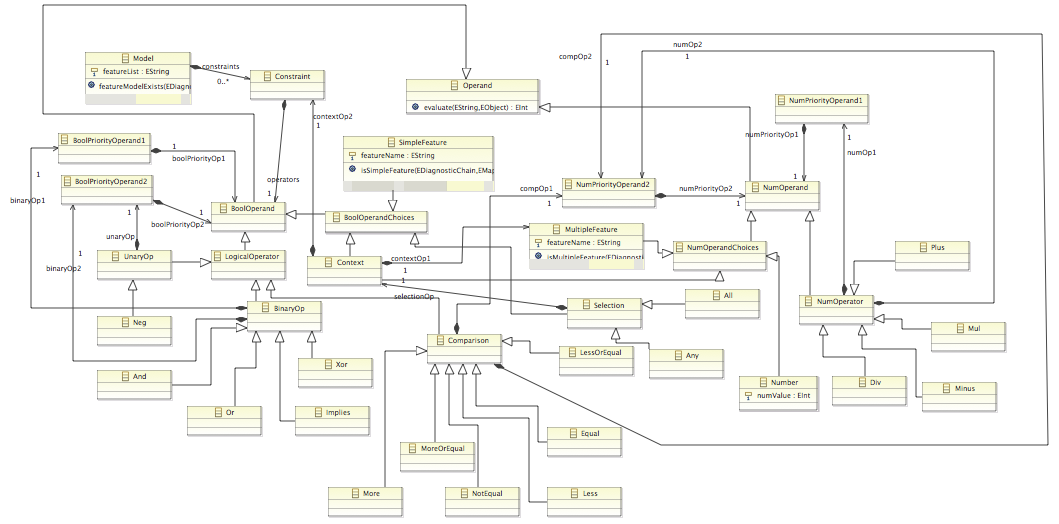
\includegraphics[scale=0.4]{metamodelo/metamodelo.jpg}
\caption{Metamodelo utilizado para la creaci�n de nuestro lenguaje de especificaci�n y validaci�n de restricciones}
\label{figmetameta}
\end{figure}


El proceso de divisi�n a partir de aqu� es m�s o menos an�logo para todas las operaciones, as� que vamos a centrarnos �nicamente en la rama que da lugar a las operaciones binarias l�gicas, para comentar despu�s los casos y situaciones especiales. Una vez tenemos la clase BoolOperand, podemos especializarla un poco m�s a LogicalOperator, que a su vez se dividir� en operaciones unarias, binarias, o de comparaci�n. Todas ellas son clases abstractas. Por fin, la clase BinaryOp heredar� las clases de las operaciones propiamente dichas, en este caso And, Or, Implies y Xor. Estas ya podr�n ser instanciadas en las sintaxis concretas que creemos.

Cabe hacer menci�n tambi�n a las clases SimpleFeature, MultipleFeature y Number, que representan a las caracter�sticas simples, m�ltiples y n�meros respectivamente. En cualquier �rbol resultante de parsear nuestro lenguaje, estas clases representar�n las hojas. En �ltima instancia todas las operaciones tendr�n como operandos caracter�sticas o n�meros. Podemos observar que SimpleFeature es un operando booleano (est� en la parte estructural de las operaciones booleanas) ya que su evaluaci�n ser� verdadero o falso, dependiendo si esa caracter�stica ha sido seleccionada en la configuraci�n correspondiente o no. MultipleFeature sin embargo se eval�a a n�mero entero. Su valor ser� el n�mero de apariciones de esa caracter�stica dentro de la configuraci�n correspondiente.

Muchas de las clases que ahora se pueden contemplar en el metamodelo de la figura \ref{figmetameta} a�n no estaban presentes en esta etapa temprana del dise�o, y su inclusi�n fue necesaria a ra�z de la creaci�n de la gram�tica y los problemas que se observaron en ese punto. En particular, las terminadas en Choices y en PriorityOperand. Las operaciones All, Any y Context en este momento eran simples herencias de BoolOperand. El motivo de estas modificaciones ser� explicado en el cap�tulo siguiente. 

Para terminar este apartado, vamos a hablar de las relaciones entre las diferentes clases de nuestro metamodelo. En este punto del dise�o no eran las mismas que las de la figura \ref{figmetameta} por los motivos explicados anteriormente. Simplemente busc�bamos una forma de relacionar cada operaci�n con los tipos de sus operandos (que tambi�n pueden ser operaciones, como es l�gico). Las operaciones l�gicas binarias tendr�n dos operandos que tambi�n ser�n binarios. En este momento del dise�o binaryOp1 y binaryOp2 iban relacionados a BoolOperand. Del mismo modo que unaryOp. Del mismo modo, compOp1, compOp2, numOp1 y numOp2 (es decir, los operandos de operaciones de comparaci�n y num�ricas respectivamente) estaban relacionados con la clase NumOperand.

La relaci�n de toda estructura de operaciones con los dos elementos anteriores, Model y Constraint, se realiza entre Constraint y BoolOperand. Toda restricci�n en �ltima ha de ser evaluada a verdadero o falso, es por eso que la relaci�n no va con Operand, como podr�a pensarse en primera instancia. De este modo estamos forzando que la operaci�n con menos profundidad del �rbol parseado de nuestra restricci�n sea booleana, y que por lo tanto el resultado final de validar la restricci�n sea un dato booleano. 

Quiz�s a alguien le pueda sorprender el hecho de que la relaci�n "operators" entre Constrain y BoolOperand sea 1..1 y no 1..*. El motivo es que como los operadores de esa primera operaci�n booleana que estamos forzando pueden ser a su vez operaciones, la complejidad en la restricci�n que podemos definir se propaga por ah� en lugar de por la relaci�n creada.







\section{Pruebas del metamodelo}
\label{sec:meta:pruebas}
%%==================================================================%%
%% Author : Tejedo Gonz�lez, Daniel                                 %%
%%          S�nchez Barreiro, Pablo                                 %%
%% Version: 1.0, 27/11/2012                                         %%                   %%                                                                  %%
%% Memoria del Proyecto Fin de Carrera                              %%
%% Gram�tica, pruebas                                       %%
%%==================================================================%%

\begin{figure}[t]
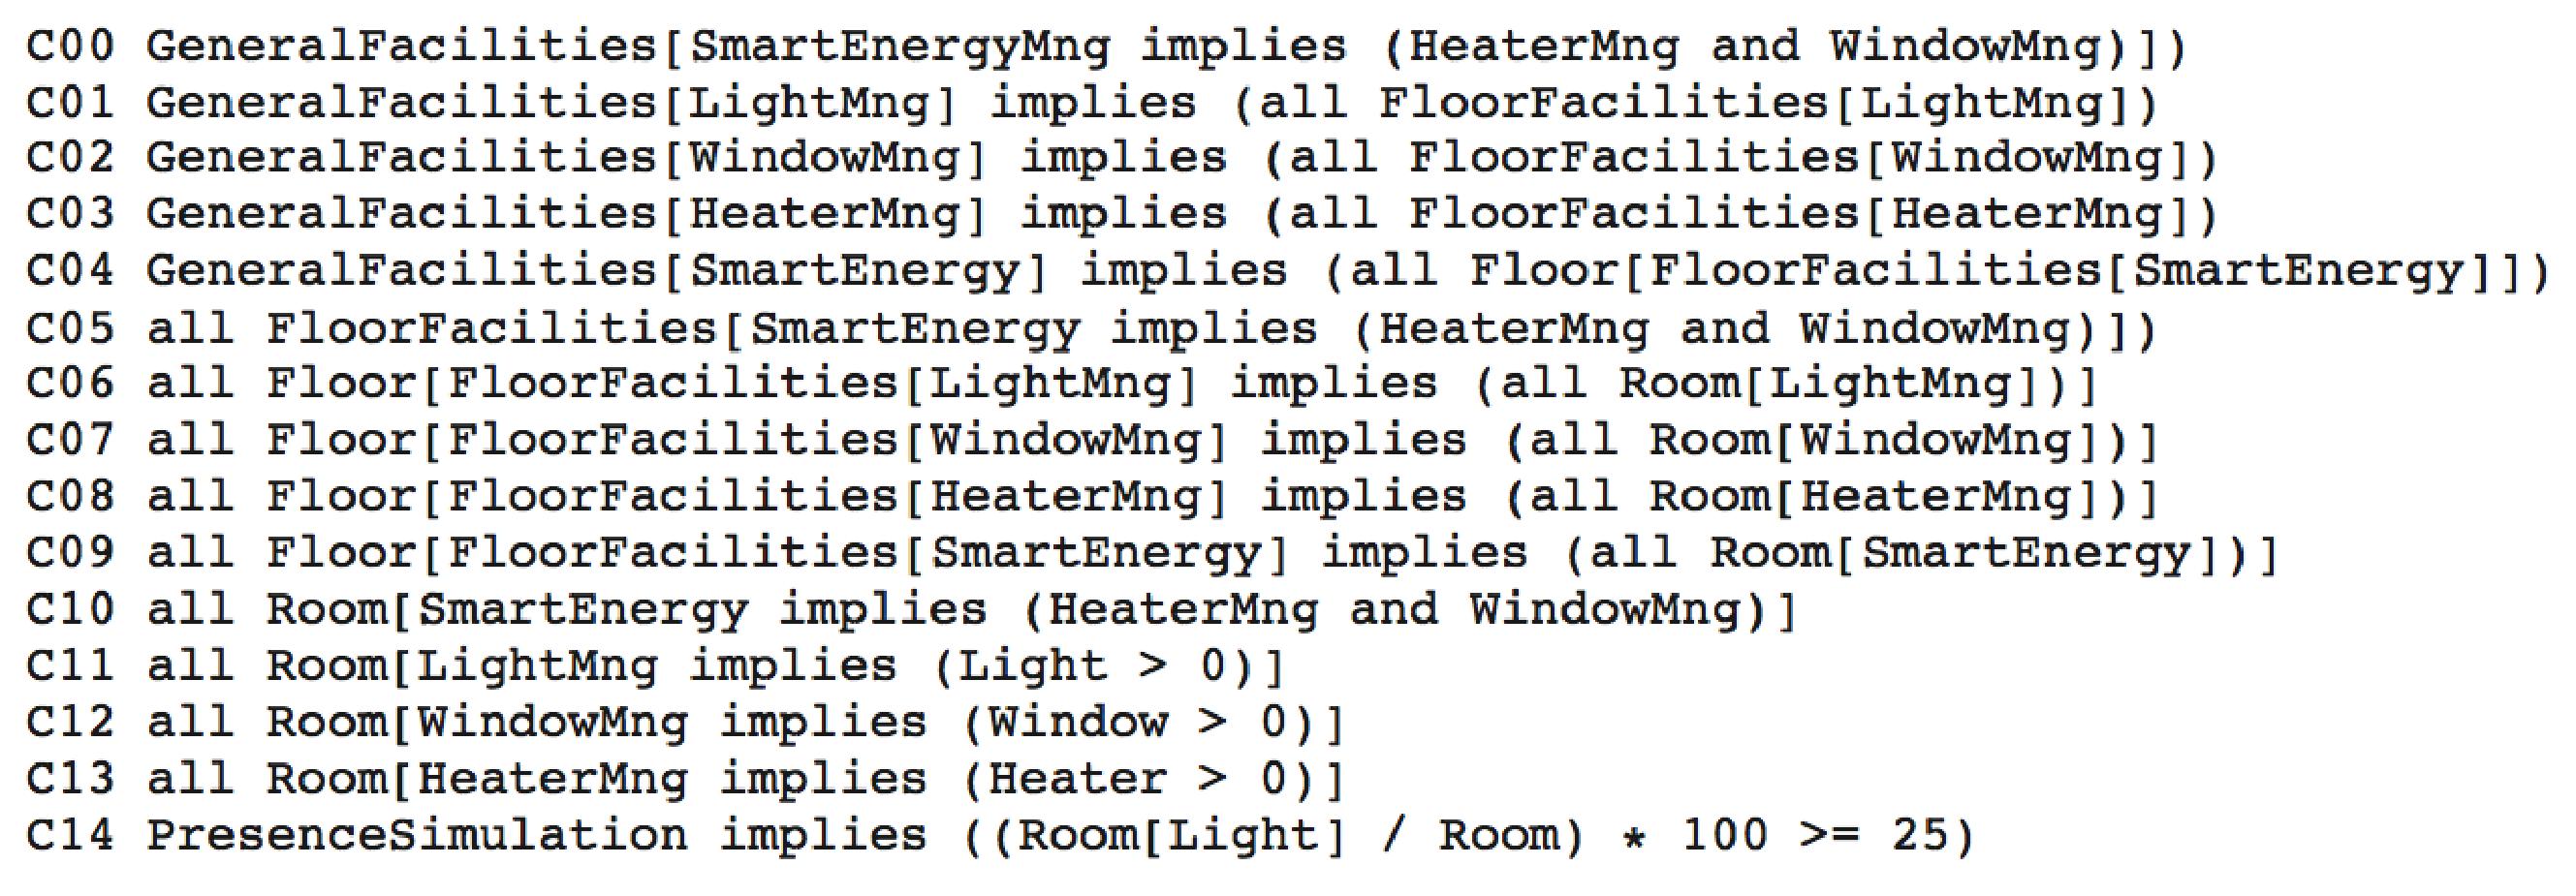
\includegraphics[scale=0.5]{gramatica/oppruebas.eps}
\caption{Bater�a de instrucciones para probar el funcionamiento de la gram�tica}
\label{figgrampruebas}
\end{figure}

Para hacer las pruebas correspondientes a la gram�tica fue de mucha utilidad la vista Outline de Eclipse, que permite obsevar el �rbol de parsing de todos los ficheros de c�digo que creemos en nuestro lenguaje. 

La bater�a de pruebas simplemente consisti� en comprobar una serie de instrucciones y observar dentro de la vista Outline si se parseaban de modo correcto. En este caso se utilizaron unas restricciones definidas en un documento previo de Hydra que conten�an todos los aspectos problem�ticos de la gram�tica, es decir, operaciones largas con prioridad y multitud de contextos. Estas instrucciones son las que se muestran en la figura \ref{figgrampruebas}. 

El resto de operaciones fueron puestas a prueba con restricciones m�s sencillitas y, como en el caso anterior, fueron exitosas. Tambi�n se usaron las instrucciones de las pruebas del cap�tulo anterior, que se pueden observar en la figura \ref{figmetains} para comprobar que el �rbol era el mismo que se cre� en ese momento.


% Cap�tulo 4: Creacion de la gramatica
%%==================================================================%%
%% Author : Tejedo Gonz�lez, Daniel                                 %%
%%          S�nchez Barreiro, Pablo                                 %%
%% Version: 1.0, 28/11/2012                                         %%                   %%                                                                  %%
%% Memoria del Proyecto Fin de Carrera                              %%
%% Validation Framework, archivo ra�z                                       %%
%%==================================================================%%

\chapterheader{Validaci�n de las sintaxis concretas}{Validaci�n de las sintaxis concretas}
\label{chap:emfvf}

Este cap�tulo trata de describir la planificaci�n que se sigui� a la hora de abordar este proyecto: metodolog�a utilizada, enumeraci�n de las diversas tareas implicadas as� como el orden en que fueron realizadas y el tiempo que fue necesario invertir para llevarlas a buen puerto.

\chaptertoc

\section{Captura de requisitos}
\label{sec:emfvf:req}
%%==================================================================%%
%% Author : Tejedo Gonz�lez, Daniel                                 %%
%%          S�nchez Barreiro, Pablo                                 %%
%% Version: 1.0, 25/11/2012                                         %%
%% Version: 2.0, 06/02/2013                                         %%
%%                                                                  %%
%% Memoria del Proyecto Fin de Carrera                              %%
%% Sintaxis abstracta, requisitos                                   %%
%%==================================================================%%

El primer paso para desarrollar nuestro lenguaje era conocer qu� aspecto deb�a tener nuestro lenguaje y qu� restricciones deb�a satisfacer. Es decir, en primer lugar debemos realizar un proceso que podemos denominar de captura de requisitos para poder comprender qu� es lo que tiene que hacer exactamente el lenguaje que se pretende crear.

Concretamente nuestro lenguaje hab�a sido pr�cticamente definido por el profesor Pablo S�nchez, del Departamento de Matem�ticas, Estad�stica y Computaci�n de la Universidad de Cantabria, mediante notaci�n BNF. Las ideas subyacentes a dicho lenguaje son las que se describen a continuaci�n.

%%==================================================================%%
%% NOTA(Pablo): Aqu� traduce la secci�n III del art�culo que te
%%              env�o adjunto. Si te hacen falta las fuentes del
%%              art�culo, me las pides.
%%
%%              Traduce primero del ingl�s y luego lo repasas y lo
%%              reescribes para que suene a castellano
%% 
%%              Si en la secci�n III no aparecen las razones por 
%%              las cuales una caracter�stica es clonable, buscar 
%%              en qu� parte del art�culo aparecen y explicarlo

%%==================================================================%%

Adem�s nuestro lenguaje deb�a permitir vincular un un modelo de caracter�sticas sobre el cual se definir�n un conjunto de restricciones externas. Este modelo se utilizar�, por ejemplo, para comprobar que los s�mbolos que aparecen como nombres de caracter�sticas en las restricciones se refieren a caracter�sticas que realmente existen en el �rbol de caracter�sticas. Por ejemplo, una restricci�n del tipo $AdvancedHeating => Heating$ carecer�a de sentido si algunas de las caracter�sticas $AdvancedHeating$ o $Heating$ no apareciesen en el �rbol de caracter�sticas sobre el cual estamos definiendo restricciones.

%%======================================================================================%%
%% NOTA(Pablo): Esto posiblemente sobre al introducir la traducci�n de la Secci�n III.
%%              Si es as�, eliminarla.
%%              Si los conceptos de restricci�n con contexto y operaci�n cuantificada
%%              no apareciesen, meter esta clasificaci�n pero resumida
%%======================================================================================%%
%%
%% De entre todos esos requisitos b�sicos, es necesario entrar en detalle en el n�mero 3
%% y enumerar la lista de operaciones que pueden ser definidas por nuestro lenguaje. Se
%% pueden clasificar en los siguientes tipos: \\
%%
%% - L�gicas: Son operaciones cuyos operandos han de ser caracter�sticas sin
%%   cardinalidad (tambi�n llamadas caracter�sticas simples), y que se evaluan a
%%   verdadero o falso. Entre las operaciones l�gicas encontramos las cl�sicas not,
%%   and, or, xor e implica.
%%
%% - Num�ricas: Sus operandos han de ser caracter�sticas con cardinalidad (tambi�n
%%   llamadas caracter�sticas m�ltiples) o simplemente n�meros. Su resultado se evalua
%%   con un valor num�rico. Las operaciones num�ricas a implementar son la suma, resta,
%%   multiplicaci�n y divisi�n.
%%
%% - Comparativas: Sus operandos han de ser caracter�sticas m�ltiples o simplemente n�meros,
%%   pero su resultado se evalua con un valor booleano. Las operaciones de comparaci�n a
%%   implementar son igual que, mayor que, menor que, distinto que, mayor o igual que y menor
%%   o igual que.
%%
%% - Operaci�n de contexto: Operaci�n que permite hacer referencia a una caracter�stica
%%   hija de otra caracter�stica. Esta operaci�n tiene sentido para seleccionar
%%   caracter�sticas cuyo nombre pueda estar repetido pero que tengan contextos diferentes.
%%   Por ejemplo, en el modelo de caracter�sticas SmartHome de la figura \ref{figsmarthome}
%%   podemos observar que la caracter�stica HeaterMng est� presente en muchos contextos
%%   diferentes. Esta operaci�n es necesaria para poder saber con seguridad a cual de esos
%%   contextos estamos aplicando la restricci�n.
%%
%% - Operaci�n de selecci�n: Operaci�n que corresponde a los operadores l�gicos cl�sicos
%%   "para todo" o "existe", y que tiene la misma funcionalidad. Evalua si una restricci�n
%%   se cumple para todos los casos en que puede existir  o si se cumple en alguno de los
%%   casos. Por ejemplo, en el modelo de la figura \ref{figsmarthome} se podr�a evaluar una
%%   restricci�n para cada una de las habitaciones que hayan sido definidas, y saber si se
%%  cumple en todas, en alguna o en ninguna.
%%
%%======================================================================================%%

Utilizando esta informaci�n como base, procedimos a crear el correspondiente metamodelo en Ecore para nuestro lenguaje.




% Cap�tulo 5: Creacion de la semantica
%%==================================================================%%
%% Author : Tejedo Gonz�lez, Daniel                                 %%
%%          S�nchez Barreiro, Pablo                                 %%
%% Version: 1.0, 28/11/2012                                         %%                   %%                                                                  %%
%% Memoria del Proyecto Fin de Carrera                              %%
%% Validation Framework, archivo ra�z                                       %%
%%==================================================================%%

\chapterheader{Validaci�n de las sintaxis concretas}{Validaci�n de las sintaxis concretas}
\label{chap:emfvf}

Este cap�tulo trata de describir la planificaci�n que se sigui� a la hora de abordar este proyecto: metodolog�a utilizada, enumeraci�n de las diversas tareas implicadas as� como el orden en que fueron realizadas y el tiempo que fue necesario invertir para llevarlas a buen puerto.

\chaptertoc

\section{Captura de requisitos}
\label{sec:emfvf:req}
%%==================================================================%%
%% Author : Tejedo Gonz�lez, Daniel                                 %%
%%          S�nchez Barreiro, Pablo                                 %%
%% Version: 1.0, 25/11/2012                                         %%
%% Version: 2.0, 06/02/2013                                         %%
%%                                                                  %%
%% Memoria del Proyecto Fin de Carrera                              %%
%% Sintaxis abstracta, requisitos                                   %%
%%==================================================================%%

El primer paso para desarrollar nuestro lenguaje era conocer qu� aspecto deb�a tener nuestro lenguaje y qu� restricciones deb�a satisfacer. Es decir, en primer lugar debemos realizar un proceso que podemos denominar de captura de requisitos para poder comprender qu� es lo que tiene que hacer exactamente el lenguaje que se pretende crear.

Concretamente nuestro lenguaje hab�a sido pr�cticamente definido por el profesor Pablo S�nchez, del Departamento de Matem�ticas, Estad�stica y Computaci�n de la Universidad de Cantabria, mediante notaci�n BNF. Las ideas subyacentes a dicho lenguaje son las que se describen a continuaci�n.

%%==================================================================%%
%% NOTA(Pablo): Aqu� traduce la secci�n III del art�culo que te
%%              env�o adjunto. Si te hacen falta las fuentes del
%%              art�culo, me las pides.
%%
%%              Traduce primero del ingl�s y luego lo repasas y lo
%%              reescribes para que suene a castellano
%% 
%%              Si en la secci�n III no aparecen las razones por 
%%              las cuales una caracter�stica es clonable, buscar 
%%              en qu� parte del art�culo aparecen y explicarlo

%%==================================================================%%

Adem�s nuestro lenguaje deb�a permitir vincular un un modelo de caracter�sticas sobre el cual se definir�n un conjunto de restricciones externas. Este modelo se utilizar�, por ejemplo, para comprobar que los s�mbolos que aparecen como nombres de caracter�sticas en las restricciones se refieren a caracter�sticas que realmente existen en el �rbol de caracter�sticas. Por ejemplo, una restricci�n del tipo $AdvancedHeating => Heating$ carecer�a de sentido si algunas de las caracter�sticas $AdvancedHeating$ o $Heating$ no apareciesen en el �rbol de caracter�sticas sobre el cual estamos definiendo restricciones.

%%======================================================================================%%
%% NOTA(Pablo): Esto posiblemente sobre al introducir la traducci�n de la Secci�n III.
%%              Si es as�, eliminarla.
%%              Si los conceptos de restricci�n con contexto y operaci�n cuantificada
%%              no apareciesen, meter esta clasificaci�n pero resumida
%%======================================================================================%%
%%
%% De entre todos esos requisitos b�sicos, es necesario entrar en detalle en el n�mero 3
%% y enumerar la lista de operaciones que pueden ser definidas por nuestro lenguaje. Se
%% pueden clasificar en los siguientes tipos: \\
%%
%% - L�gicas: Son operaciones cuyos operandos han de ser caracter�sticas sin
%%   cardinalidad (tambi�n llamadas caracter�sticas simples), y que se evaluan a
%%   verdadero o falso. Entre las operaciones l�gicas encontramos las cl�sicas not,
%%   and, or, xor e implica.
%%
%% - Num�ricas: Sus operandos han de ser caracter�sticas con cardinalidad (tambi�n
%%   llamadas caracter�sticas m�ltiples) o simplemente n�meros. Su resultado se evalua
%%   con un valor num�rico. Las operaciones num�ricas a implementar son la suma, resta,
%%   multiplicaci�n y divisi�n.
%%
%% - Comparativas: Sus operandos han de ser caracter�sticas m�ltiples o simplemente n�meros,
%%   pero su resultado se evalua con un valor booleano. Las operaciones de comparaci�n a
%%   implementar son igual que, mayor que, menor que, distinto que, mayor o igual que y menor
%%   o igual que.
%%
%% - Operaci�n de contexto: Operaci�n que permite hacer referencia a una caracter�stica
%%   hija de otra caracter�stica. Esta operaci�n tiene sentido para seleccionar
%%   caracter�sticas cuyo nombre pueda estar repetido pero que tengan contextos diferentes.
%%   Por ejemplo, en el modelo de caracter�sticas SmartHome de la figura \ref{figsmarthome}
%%   podemos observar que la caracter�stica HeaterMng est� presente en muchos contextos
%%   diferentes. Esta operaci�n es necesaria para poder saber con seguridad a cual de esos
%%   contextos estamos aplicando la restricci�n.
%%
%% - Operaci�n de selecci�n: Operaci�n que corresponde a los operadores l�gicos cl�sicos
%%   "para todo" o "existe", y que tiene la misma funcionalidad. Evalua si una restricci�n
%%   se cumple para todos los casos en que puede existir  o si se cumple en alguno de los
%%   casos. Por ejemplo, en el modelo de la figura \ref{figsmarthome} se podr�a evaluar una
%%   restricci�n para cada una de las habitaciones que hayan sido definidas, y saber si se
%%  cumple en todas, en alguna o en ninguna.
%%
%%======================================================================================%%

Utilizando esta informaci�n como base, procedimos a crear el correspondiente metamodelo en Ecore para nuestro lenguaje.




% Cap�tulo 6: Conclusiones y Trabajos Futuros
%%==================================================================%%
%% Author : Tejedo Gonz�lez, Daniel                                 %%
%%          S�nchez Barreiro, Pablo                                 %%
%% Version: 1.0, 28/11/2012                                         %%                   %%                                                                  %%
%% Memoria del Proyecto Fin de Carrera                              %%
%% Validation Framework, archivo ra�z                                       %%
%%==================================================================%%

\chapterheader{Validaci�n de las sintaxis concretas}{Validaci�n de las sintaxis concretas}
\label{chap:emfvf}

Este cap�tulo trata de describir la planificaci�n que se sigui� a la hora de abordar este proyecto: metodolog�a utilizada, enumeraci�n de las diversas tareas implicadas as� como el orden en que fueron realizadas y el tiempo que fue necesario invertir para llevarlas a buen puerto.

\chaptertoc

\section{Captura de requisitos}
\label{sec:emfvf:req}
%%==================================================================%%
%% Author : Tejedo Gonz�lez, Daniel                                 %%
%%          S�nchez Barreiro, Pablo                                 %%
%% Version: 1.0, 25/11/2012                                         %%
%% Version: 2.0, 06/02/2013                                         %%
%%                                                                  %%
%% Memoria del Proyecto Fin de Carrera                              %%
%% Sintaxis abstracta, requisitos                                   %%
%%==================================================================%%

El primer paso para desarrollar nuestro lenguaje era conocer qu� aspecto deb�a tener nuestro lenguaje y qu� restricciones deb�a satisfacer. Es decir, en primer lugar debemos realizar un proceso que podemos denominar de captura de requisitos para poder comprender qu� es lo que tiene que hacer exactamente el lenguaje que se pretende crear.

Concretamente nuestro lenguaje hab�a sido pr�cticamente definido por el profesor Pablo S�nchez, del Departamento de Matem�ticas, Estad�stica y Computaci�n de la Universidad de Cantabria, mediante notaci�n BNF. Las ideas subyacentes a dicho lenguaje son las que se describen a continuaci�n.

%%==================================================================%%
%% NOTA(Pablo): Aqu� traduce la secci�n III del art�culo que te
%%              env�o adjunto. Si te hacen falta las fuentes del
%%              art�culo, me las pides.
%%
%%              Traduce primero del ingl�s y luego lo repasas y lo
%%              reescribes para que suene a castellano
%% 
%%              Si en la secci�n III no aparecen las razones por 
%%              las cuales una caracter�stica es clonable, buscar 
%%              en qu� parte del art�culo aparecen y explicarlo

%%==================================================================%%

Adem�s nuestro lenguaje deb�a permitir vincular un un modelo de caracter�sticas sobre el cual se definir�n un conjunto de restricciones externas. Este modelo se utilizar�, por ejemplo, para comprobar que los s�mbolos que aparecen como nombres de caracter�sticas en las restricciones se refieren a caracter�sticas que realmente existen en el �rbol de caracter�sticas. Por ejemplo, una restricci�n del tipo $AdvancedHeating => Heating$ carecer�a de sentido si algunas de las caracter�sticas $AdvancedHeating$ o $Heating$ no apareciesen en el �rbol de caracter�sticas sobre el cual estamos definiendo restricciones.

%%======================================================================================%%
%% NOTA(Pablo): Esto posiblemente sobre al introducir la traducci�n de la Secci�n III.
%%              Si es as�, eliminarla.
%%              Si los conceptos de restricci�n con contexto y operaci�n cuantificada
%%              no apareciesen, meter esta clasificaci�n pero resumida
%%======================================================================================%%
%%
%% De entre todos esos requisitos b�sicos, es necesario entrar en detalle en el n�mero 3
%% y enumerar la lista de operaciones que pueden ser definidas por nuestro lenguaje. Se
%% pueden clasificar en los siguientes tipos: \\
%%
%% - L�gicas: Son operaciones cuyos operandos han de ser caracter�sticas sin
%%   cardinalidad (tambi�n llamadas caracter�sticas simples), y que se evaluan a
%%   verdadero o falso. Entre las operaciones l�gicas encontramos las cl�sicas not,
%%   and, or, xor e implica.
%%
%% - Num�ricas: Sus operandos han de ser caracter�sticas con cardinalidad (tambi�n
%%   llamadas caracter�sticas m�ltiples) o simplemente n�meros. Su resultado se evalua
%%   con un valor num�rico. Las operaciones num�ricas a implementar son la suma, resta,
%%   multiplicaci�n y divisi�n.
%%
%% - Comparativas: Sus operandos han de ser caracter�sticas m�ltiples o simplemente n�meros,
%%   pero su resultado se evalua con un valor booleano. Las operaciones de comparaci�n a
%%   implementar son igual que, mayor que, menor que, distinto que, mayor o igual que y menor
%%   o igual que.
%%
%% - Operaci�n de contexto: Operaci�n que permite hacer referencia a una caracter�stica
%%   hija de otra caracter�stica. Esta operaci�n tiene sentido para seleccionar
%%   caracter�sticas cuyo nombre pueda estar repetido pero que tengan contextos diferentes.
%%   Por ejemplo, en el modelo de caracter�sticas SmartHome de la figura \ref{figsmarthome}
%%   podemos observar que la caracter�stica HeaterMng est� presente en muchos contextos
%%   diferentes. Esta operaci�n es necesaria para poder saber con seguridad a cual de esos
%%   contextos estamos aplicando la restricci�n.
%%
%% - Operaci�n de selecci�n: Operaci�n que corresponde a los operadores l�gicos cl�sicos
%%   "para todo" o "existe", y que tiene la misma funcionalidad. Evalua si una restricci�n
%%   se cumple para todos los casos en que puede existir  o si se cumple en alguno de los
%%   casos. Por ejemplo, en el modelo de la figura \ref{figsmarthome} se podr�a evaluar una
%%   restricci�n para cada una de las habitaciones que hayan sido definidas, y saber si se
%%  cumple en todas, en alguna o en ninguna.
%%
%%======================================================================================%%

Utilizando esta informaci�n como base, procedimos a crear el correspondiente metamodelo en Ecore para nuestro lenguaje.




% CONTENT: Appendices, if desired
% \renewcommand\chaptername{Appendix}                      % hereafter, chapters are called "Appendix"
\renewcommand\thechapter{\Alph{chapter}}        % chapter number in Romans
\renewcommand\thesection{\Alph{chapter}.\alph{section}}  % make sections "I.a", instead of "1.1"
\setcounter{chapter}{0}                                  % start numbering chapters from 1 on again


% Appendix A:
% \input{populo/populo.tex} % Appendix I

% CONFIG: Bibliography style
\cleardoublepage                            % start in right side page
\addcontentsline{toc}{chapter}{References}  % add this "chapter" to the ToC, with the name "Bibliography"
%\bibliographystyle{alpha}                  % bibliography style
\bibliographystyle{abbrv}                  % bibliography style
\bibliography{references/references.bib}

\end{document}
